%%%%%%%%%%%%%%%%%%%%%%%%%%%%%%%%%%%%%%%%%%%%%%%%%%%%%%%%%%%%%%%%%%%%%%%%%%%%%%%%%%%%%%%%%%%%%%%%%%%%%%%%%%%%%%%%%%%%%%%%%%%%%%%%%%%%%%%%%%%%%%%%%%%%%%%%%%%
% This is just an example/guide for you to refer to when submitting manuscripts to Frontiers, it is not mandatory to use Frontiers .cls files nor frontiers.tex  %
% This will only generate the Manuscript, the final article will be typeset by Frontiers after acceptance.   
% When submitting your files, remember to upload this *tex file, the pdf generated with it, the *bib file (if bibliography is not within the *tex) and all the figures.
%%%%%%%%%%%%%%%%%%%%%%%%%%%%%%%%%%%%%%%%%%%%%%%%%%%%%%%%%%%%%%%%%%%%%%%%%%%%%%%%%%%%%%%%%%%%%%%%%%%%%%%%%%%%%%%%%%%%%%%%%%%%%%%%%%%%%%%%%%%%%%%%%%%%%%%%%%%

%%% Version 3.4 Generated 2018/06/15 %%%
%%% You will need to have the following packages installed: datetime, fmtcount, etoolbox, fcprefix, which are normally inlcuded in WinEdt. %%%
%%% In http://www.ctan.org/ you can find the packages and how to install them, if necessary. %%%
%%%  NB logo1.jpg is required in the path in order to correctly compile front page header %%%

\documentclass[utf8]{frontiersSCNS} % for Science, Engineering and Humanities and Social Sciences articles
%\documentclass[utf8]{frontiersHLTH} % for Health articles
%\documentclass[utf8]{frontiersFPHY} % for Physics and Applied Mathematics and Statistics articles

%\setcitestyle{square} % for Physics and Applied Mathematics and Statistics articles
\usepackage{url,hyperref,lineno,microtype,subcaption}
\usepackage[onehalfspacing]{setspace}
\usepackage{xr}
% \usepackage{geometry}
\usepackage{pdflscape}
\usepackage{titlesec}
% In your preamble
\usepackage{textcomp}
\titlespacing*{\subsubsection}
{0pt}{1ex}{1ex}
\titlespacing*{\subsection}
{0pt}{2ex}{2ex}
\hypersetup{pdfborder = {0 0 0}}

\usepackage{cleveref}
\makeatletter
\newcommand*{\addFileDependency}[1]{% argument=file name and extension
  \typeout{(#1)}
  \@addtofilelist{#1}
  \IfFileExists{#1}{}{\typeout{No file #1.}}
}
\makeatother

\newcommand*{\myexternaldocument}[1]{%
    \externaldocument{#1}%
    \addFileDependency{#1.tex}%
    \addFileDependency{#1.aux}%
}

\myexternaldocument{frontiers_SupplementaryMaterial}

\linenumbers


% Leave a blank line between paragraphs instead of using \\


\def\keyFont{\fontsize{8}{11}\helveticabold }
\def\firstAuthorLast{McParland {et~al.}} %use et al only if is more than 1 author
\def\Authors{Erin L. McParland\,$^{1,*}$, Harriet Alexander\,$^{2, *}$ and Winifred M. Johnson\,$^{3, *}$}
% Affiliations should be keyed to the author's name with superscript numbers and be listed as follows: Laboratory, Institute, Department, Organization, City, State abbreviation (USA, Canada, Australia), and Country (without detailed address information such as city zip codes or street names).
% If one of the authors has a change of address, list the new address below the correspondence details using a superscript symbol and use the same symbol to indicate the author in the author list.
\def\Address{$^{1}$Department of Marine Chemistry and Geochemistry, Woods Hole Oceanographic Institution, Woods Hole, MA, USA \\
$^{2}$Biology Department, Woods Hole Oceanographic Institution, Woods Hole, MA, USA\\
$^{3}$Department of Chemistry and Biochemistry, University of North Carolina Wilmington, Wilmington, NC, USA}
% The Corresponding Author should be marked with an asterisk
% Provide the exact contact address (this time including street name and city zip code) and email of the corresponding author
\def\corrAuthor{Winifred Johnson}

\def\corrEmail{johnsonwm@uncw.edu}




\begin{document}
\onecolumn
\firstpage{1}

\title[Marine osmolytes]{The osmolyte ties that bind: genomic insights into synthesis and breakdown of organic osmolytes in marine microbes} 

\author[\firstAuthorLast ]{\Authors} %This field will be automatically populated
\address{} %This field will be automatically populated
\correspondance{} %This field will be automatically populated

% \extraAuth{}% If there are more than 1 corresponding author, comment this line and uncomment the next one.
\extraAuth{Harriet Alexander \\ halexander@whoi.edu \\ Erin L. McParland \\ emcparland@whoi.edu }


\maketitle


\begin{abstract}

%%% Leave the Abstract empty if your article does not require one, please see the Summary Table for full details.
\section{}

%Marine phytoplankton make up only {\raise.17ex\hbox{$\scriptstyle\sim$}}1-2\% of global plant biomass, yet they are responsible for approximately 40\% of global carbon fixation. About 50\% of this fixed carbon is consumed by heterotrophic bacteria each day, representing a large global flux of energy and matter. Labile organic compounds (metabolites) are the primary supply of marine heterotrophs’ energetic and nutritional demands, but these compounds remain elusive because of their rapid turnover and concomitant minuscule concentrations in the dissolved organic matter pool. 
The production and consumption of organic matter by marine organisms plays a central role in the marine carbon cycle. Labile organic compounds (metabolites) are the major currency of energetic demands and organismal interaction, but these compounds remain elusive because of their rapid turnover and concomitant minuscule concentrations in the dissolved organic matter pool. Organic osmolytes are a group of small metabolites synthesized at high intracellular concentrations (mM) to regulate cellular osmolarity and have the potential to be released as abundant dissolved substrates. Osmolytes may represent an essential currency of exchange among heterotrophic prokaryotes and primary and secondary producers in marine food webs. For example, the well-known metabolite dimethylsulfoniopropionate (DMSP) is used as an osmolyte by some phytoplankton and can be subsequently metabolized by 60\% of the marine bacterial community, supplying up to 13\% of the bacterial carbon demand and 100\% of the bacterial sulfur demand. While marine osmolytes have been studied for decades, our understanding of their cycling and significance within microbial communities is still far from comprehensive. 

Here, we surveyed the genes responsible for synthesis, breakdown, and transport of 14 key osmolytes. We systematically searched for these genes across marine bacterial genomes (n = 897) and protistan transcriptomes (n = 652) using homologous protein profiles to investigate the potential for osmolyte metabolisms. Using the pattern of gene presence and absence, we infer the metabolic potential of surveyed microbes to interact with each osmolyte. Specifically, we identify: 1) complete pathways for osmolyte synthesis in both prokaryotic and eukaryotic marine microbes, 2) microbes capable of transporting osmolytes but lacking complete synthesis and/or breakdown pathways, and 3) osmolytes whose synthesis and/or breakdown appears to be specialized and is limited to a subset of organisms. The analysis clearly demonstrates that the marine microbial loop has the genetic potential to actively recycle osmolytes and that this abundant group of small metabolites may function as a significant source of nutrients through exchange among diverse microbial groups that significantly contribute to the cycling of labile carbon.

\tiny
 \keyFont{ \section{Keywords:} osmolytes, glycine betaine, mannitol, transporters, biosynthesis, catabolism, metatranscriptomics} %All article types: you may provide up to 8 keywords; at least 5 are mandatory.
\end{abstract}

\section{Introduction}

Marine microbes live in a high salinity environment and must maintain cellular mechanisms for rapid response to any small changes in external water potential in order to maintain cellular homeostasis \citep{Bisson1995}. Ions are most readily transported by microbes, and therefore their concentrations typically respond first to external salinity changes. However, the charged nature of ions can only be tolerated by cellular physiology at specific concentrations, and ions are most often stored in solution within vacuoles in phytoplankton. Thus, organic osmolytes represent a critical addition to cellular osmotic balance. Throughout the rest of this paper when we refer to osmolytes, we will be exclusively discussing organic osmolytes. Osmolytes are often referred to as compatible solutes as they are small, organic molecules that are highly soluble and can accumulate at high concentrations within the cytoplasm without interfering with cellular function \citep{Roebler2001,Stefels2000}. Although organic osmolytes are energetically more costly to use than inorganic ions, because they must be either synthesized or actively transported into the cell, many serve multiple functions in addition to their osmotic contributions. Osmolytes have been shown to contribute to protein stabilization and to have other cytoprotective properties under salinity, temperature, and pressure stress \citep{Kirst1989,Ma2017,Yancey2015,Burg2008}. Some osmolytes have been shown to be efficient scavengers of reactive oxygen species \citep{Smirnoff1989,Sunda2002,Brands2019}. Osmolytes have also been predicted to function in a ballasting mechanism, where the synthesis of osmolytes with different densities would alter cellular buoyancy \citep{Boyd2002,Lavoie2015}. Osmolytes have been of interest in the marine context for decades \citep{Challenger1951,Yancey1982,Kiene1998,Keller1999}. However, with the exception of a few extensively studied osmolytes (e.g. dimethylsulfoniopropionate (DMSP)), we know relatively little about osmolyte distributions in the ocean, the role of environmental conditions in controlling intracellular osmolyte abundances and subsequent release into the dissolved phase, or the significance of osmolytes as substrates in the microbial loop.

In marine systems, a range of amino acids and their derivatives, carbohydrates, methylsulfonium compounds, and methylammonium compounds have been identified as osmolytes used by marine organisms ranging from bacteria to tube worms \citep{Yancey2005} (\Cref{tabl:osmodiss}). All macro- and microalgae exhibit the ability to accumulate both inorganic ions and organic osmolytes \citep{Bisson1995}, though their salinity tolerances have been shown to be a function of the isolation location's salinity conditions (open ocean vs. coastal ocean) \citep{Brand1984,Kirst1989}. In general, phytoplankton contain one or two major organic osmolytes with concentrations $> 50mM$, and many minor organic osmolytes with concentrations $< 5mM$ \citep{Gebser2013}. However, monoculture studies have demonstrated that the composition of organic osmolytes is variable and strongly taxa dependent \citep{Dickson1987,Dickson1987.2}. Marine phytoplankton use many well-known plant osmolytes \citep{Yancey2005}, but also osmolytes that are primarily found in the marine environment. For example, DMSP is found in a diverse array of marine phytoplankton, and was originally described as an osmolyte due to its similar structure to glycine betaine \citep{Andreae1986}. DMSP is hypothesized to be multi-functional, but likely functions predominantly as an osmolyte in dinoflagellate and haptophyte groups which typically contain $>50mM$ intracellular DMSP \citep{Keller1989,Stefels2000,McParland2020}. 2,3-dihydroxypropane-1-sulfonate (DHPS) was very recently reported to be present at osmolyte-like concentrations in some diatoms ($15mM$) and coccolithophores ($18mM$) \citep{Durham2019}, and its intracellular concentrations in the Antarctic sea-ice diatom \emph{Nitzschia lecointei} ($\sim 85mM$) correlate with salinity and temperature changes \citep{Dawson2020}. Some marine diatoms have also been shown to be capable of transporting ectoine or DMSP for osmotic functions \citep{Spielmeyer2011,Lavoie2018,Fenizia2020}. Across prokaryotes, halophilic archaea and bacteria have uniquely adapted cellular machinery that can withstand molar concentrations of potassium and chloride ions \citep{Roebler2001}, but most marine prokaryotes also utilize organic osmolytes. Some prokaryotes maintain \emph{de novo} synthesis pathways, while many others are capable of transporting osmolytes available in the dissolved pool \citep{Poli2017,Poretsky2010}. Two well-known marine nitrogen-fixing Cyanobacteria use different organic osmolytes from each other: \emph{Crocosphaera} synthesizes trehalose, while \emph{Trichodesmium} synthesizes homoserine betaine \citep{Pade2012,Pade2016}. The chemoautotroph \emph{Sulfurimonas} was recently shown to synthesize proline with increasing salinity \citep{Gotz2018}, while \emph{Vibrio parahaemolyticus} synthesizes ectoine as an osmolyte \citep{Ongagna-Yhombi2013}. Rather than synthesizing osmolytes \emph{de novo}, prokaryotes can also transport and retain them under salinity stress. For example, uptake of radiolabeled DMSP and glycine betaine by natural communities of bacterioplankton has been shown to increase with salinity, and a significant proportion of the spiked osmolytes remained untransformed after uptake \citep{Kiene1998,Motard-Cote2015}.

Osmolytes are some of the most concentrated (mM) small molecules in marine microbes, and therefore have the potential to be released as abundant carbon substrates to the dissolved organic matter (DOM) pool. The small size of osmolytes make them inherently labile substrates compared to larger biopolymers, such as proteins, polysaccharides, and lipids, which require additional extracellular processing. Uptake studies of DMSP, glycine betaine, and taurine have estimated that these molecules provide up to 13\% \citep{Kiene2000}, 38\% \citep{Kiene1998}, or 4\% \citep{Clifford2020} of bacterial carbon demand, respectively. When we consider the scale of the global carbon flux that is used by bacterioplankton (50\% of net primary productivity \citep{Ducklow2000}), these substrates could contribute monumentally to this flux of energy and matter and dictate relationships amongst organisms. Catabolic pathways for other osmolytes, such as those identified for ectoine and 5-hydroxyectoine in the marine bacterium, \emph{Ruegeria pomeroyi}, indicate that other osmolytes could also be valuable substrates \citep{Schulz2017}, but lack relevant environmental measurements to quantify their abundance and role within the microbial loop.

Previous measurements of osmolytes within DOM range from $\sim pM - nM$ concentrations (\Cref{tabl:osmodiss}), which contrast with the $mM$ intracellular concentrations of osmolytes, suggesting that osmolytes are rapidly consumed upon release to the dissolved pool. As osmolyte concentrations can approach limits of detection with current analytical techniques, the down-regulation of transcripts associated with osmolyte consumption have been quantified as a proxy for utilization \citep{Vorobev2018}. When applying this technique to natural communities, the osmolytes glycine betaine, mannitol, taurine, proline, and sorbitol were all predicted to be rapidly recycled in less than 24 hours \citep{Vorobev2018}. Osmolyte concentrations and availability have been hypothesized to be a function of both community composition and other environmental drivers. For example, DMSP concentrations were predicted to be determined by phytoplankton community composition \citep{McParland2019}. Recent analytical advances have expanded our knowledge to a wide array of osmolytes and their environmental variability (including trehalose, sucrose, glucosylglycerol, DHPS, DMSP, glycine betaine, proline, homarine). Particulate abundances of some osmolytes are linked to diel cycles \citep{Boysen2020}, and different osmolytes dominate on sinking particles (glycine betaine, proline) compared to suspended particles (i.e. planktonic cells; DMSP) \citep{Johnson2020}. Although extensive measurements of DMSP concentrations and turnover rates exist \citep{Kiene2000}, the dissolved concentrations and turnover rates of most marine osmolytes are unknown  (\Cref{tabl:osmodiss}) and require further experimental work to fully understand the factors that drive their distributions.

In this study, we explored the role of osmolytes within the marine microbial loop by identifying microbes with the potential to synthesize, catabolize, assimilate, or transport osmolytes. We hypothesized that different patterns of osmolyte metabolisms would reveal the role of osmolytes as valuable nutrients (i.e. potential carbon, nitrogen, and/or sulfur substrates) in the microbial loop. We first explored the taxonomic trends of potential producers and consumers by surveying osmolyte synthesis and utilization in genomes and transcriptomes from monocultures. We then compared these results with \emph{in situ} transcription of mannitol and glycine betaine transport, synthesis, and breakdown in the Tara metatranscriptomes from the surface ocean. 

\section{Materials and Methods}

\subsection{Manual curation of osmolyte-related KEGG orthologs}

Osmolytes (n = 23) were initially selected for investigation based on their ubiquity within microorganisms or their previously identified importance in marine systems (\Cref{tabl:osmodiss}). We chose to use the Kyoto Encyclopedia of Genes and Genomes (KEGG) as the database from which to identify metabolic pathways associated with the osmolytes and the corresponding gene orthologs, referred to as KEGG orthologs (KOs) throughout this paper \citep{Kanehisa2000,Kanehisa2012}. Only 18 of these osmolytes of interest were metabolites mapped in KEGG. In addition, glucosylglycerol had to be excluded because there were no genes associated with this compound in KEGG and trigonelline was also excluded due to missing KOs in the pathway available on KEGG. Dimethylsulfoniopropionate (DMSP) was also removed from the list of osmolytes considered because the pathways involved in its biosynthesis and breakdown are incomplete in KEGG. Finally, hydroxyectoine was not analyzed in detail as it is a closely linked derivative of ectoine. Thus, our analysis was performed on 14 osmolytes (\Cref{tabl:pathnum}).

The KOs associated with the synthesis, breakdown, and transport of these metabolites were manually compiled (Supplemental Data Sheet 1). We sought to identify synthesis pathways that began with a common metabolite, such as a sugar or amino acid, rather than an intermediate. Similarly, we mapped breakdown pathways to endpoints that could be incorporated back into metabolism for either catabolic or anabolic purposes. Transporters are not comprehensively represented in KEGG and thus we chose to focus on the available ABC transporters. This limited us to transporters for glycerol, glycine betaine, mannitol, sorbitol, and taurine. By mapping the pathways in this way, we sought to identify organisms that could use ubiquitous building blocks to synthesize an osmolyte and those who could breakdown an osmolyte into biologically relevant molecules that could be used for another metabolic purpose.

To facilitate identification of synthesis and breakdown capabilities in organisms, we identified each of the genes required for a selected pathway by numerically labeling each gene as a step in a pathway as well as indicating alternative complete pathways (Supplemental Data Sheet 1). Finally, we created a comprehensive list of the KOs associated with synthesis, breakdown, and transport for each osmolyte to use in downstream homology searches. This resulted in 482 possible reactions or transporter components, but included replicate KOs because some pathways required the same KO as another pathway at certain steps. Ultimately, 486 unique KOs were identified (Supplemental Data Sheet 2). To confirm that our manual curation had comprehensively captured the genes associated with each osmolyte according to KEGG, we computationally searched a list of KOs directly associated with each osmolyte and checked this list against our manually curated pathways.

\subsection{Homolog searching of KEGG orthologs against marine prokaryotic genomes and eukaryotic protistan transcriptomes}

Genomes from representative marine bacteria and archaea were collected from MarRef (v5) (n = 897) \citep{ten_Hoopen_2017,Klemetsen_2017}, and transcriptomes from representative marine protists were collected from the Marine Microbial Eukaryotic Transcriptome Sequencing Project (MMETSP) (n = 652) \citep{Johnson_2018, Keeling_2014} (Supplemental Data Sheet 2). The predicted proteins from both the prokaryotic genomes and MMETSP transcriptomes were used in the subsequent analyses. All 486 KOs that were identified through manual curation as associated with the metabolic processing or transport of key osmolytes (\Cref{tabl:pathnum}) were searched against the predicted proteins from the MMETSP and MarRef datasets. A snakemake pipeline (v. 5.24.2) \citep{M_lder_2021} based off of kofamscan \citep{Aramaki_2019, Mistry_2013} was built to search for the likely presence of the osmolyte-related KOs in our protein sets of interest. KO hmm profiles were downloaded from KEGG (\url{https://www.genome.jp/tools/kofamkoala/}) on October 6, 2020. Both the MarRef and MMETSP predicted protein sets were searched for a given KO with hmmsearch (HMMER v. 3.3.1). True hits for KOs were parsed from the resulting hmm output with a custom script (parse\_hmmsearch.py) run with python v. 3.9.1 and biopython v. 1.78 \citep{Cock_2009}, which parses hits based on the adaptive bitscore cutoff values used by \texttt{kofamscan} as published in the \texttt{ko\_list} file \citep{Aramaki_2019}. A final table with presence or absence of all osmolyte-related KOs for each organism was generated (Supplemental Data Sheet 2). This pipeline and all associated scripts and analysis notebooks is available as a GitHub repo (\url{https://github.com/AlexanderLabWHOI/2021-marine-osmolytes}). 

\subsection{Metabolic potential prediction}

Using the manually curated pathway listings (Supplemental Data Sheet 1), a python based script was used to identify the presence or absence of a given metabolic pathway associated with the synthesis, breakdown, or transport for an organism (Supplemental Data Sheet 3). To be considered capable of osmolyte synthesis or breakdown, an organism was required to have at least one complete pathway between the identified common metabolite (as described above). In cases where a pathway had more than one step (\Cref{tabl:pathnum}), the organism had to have all steps present for it to be annotated as capable of synthesis or breakdown. In cases where a step was identified on a pathway map, but was not annotated with a KO, the pathway was not considered. For the annotation of transporters, genomes were required to contain all KOs (subunits) of a given transporter to be annotated as capable of transport. In the case of glycine betaine, which contains two different transport pathways, only one transporter system was required to be present to confer the ability to transport. 

\subsection{Prokaryotic phylogeny comparison}

Phylogenetic trees from the MarRef genomes were constructed using GToTree v1.4.7 \citep{Lee_2019, Price_2010}. Trees were constructed with the `Universal` dataset of 15 genes as defined by \citet{Hug_2016} and default parameters. Trees were visualized using iTOL  \citep{Letunic_2016} and the presence or absence of synthesis, breakdown, and transport capabilities were visualized across all genomes and publication-quality figures were generated. 


\subsection{Identifying orthologs in Tara Oceans}

To assess the potential importance of osmolyte metabolic processes across the global ocean, KOs from genes associated with glycine betaine and mannitol synthesis, breakdown, and transport were searched against the surface data from the Tara Oceans dataset using the Tara Oceans Gene Atlas \citep{Villar_2018}. A selenium-based web bot was used to automate the search submission and result download process (\url{https://github.com/AlexanderLabWHOI/2021-marine-osmolytes/tree/master/genome-searching/tara-scraping}). KO file hmm profiles from kofamscan were uploaded to Tara Ocean gene atlas and searched against the metagenome and metatranscriptome datatsets for both the the `eukaryotic` dataset, Marine Atlas of Tara Oceans Unigenes (MATOU v1) \citep{Carradec2018}, and Marine Atlas of Tara Oceans Unigenes and the `prokaryotic` dataset, Ocean Microbial Reference Gene Catalog (OM-RGC v2, including the Arctic dataset) \citep{Salazar_2019}. All searches were initially run with a generous e-value cutoff of 1e-10 and all count-based data were returned as "percent of mapped reads". We filtered the returned alignment files to retain only orthologs which passed the identified bitscore cutoff from kofamscan (Supplemental Data Sheet 4), such as we used in our genomic and transcriptomic analyses above. Notably, these cutoff values are quite stringent and significantly reduced the number of hits we reported (Supplemental Data Sheet 4). It is likely that assembled metagenomic or metatranscriptomic orthologs that are incomplete were not included in the analysis, but we believe this conservative cutoff best reflects true hits in the Tara dataset. Taxonomic annotation of orthologs recovered was assessed using the reported taxonomy from Ocean Gene Atlas. 

\subsection{Plotting and statistical analysis}

Data was analyzed and figures were generated with matplotlib v. 3.3.1 \citep{Hunter:2007}, pandas v. 1.1.2 \citep{reback2020pandas}, and seaborn v. 0.11.0 \citep{waskom2020seaborn}. Spearman correlations were calculated with the stats.spearmanr function within scipy v. 1.5.2 \citep{2020SciPy-NMeth}. Multi-testing p-value correction was done with the \texttt{multipletests} function within statsmodels 0.12.1 using the Bonferroni method. Global map distributions were plotted using cartopy 0.18.0 \citep{Cartopy}.

\section{Results and Discussion}

\subsection{Osmolyte synthesis, breakdown, and transport in marine prokaryote and eukaryote monocultures}

In this study, we manually curated the genes responsible for the synthesis, breakdown, and transport of marine osmolytes (n = 14) (\Cref{tabl:osmodiss} \& \ref{tabl:pathnum}) that are classified as either amino acids and their derivatives (n = 8), sugars (n = 5), or an amine oxide (n = 1). We then assessed the presence of these osmolyte-associated genes across marine prokaryotic genomes (MarRef) and marine eukaryotic transcriptomes from protists (MMETSP). The MarRef genomes (n = 897) contain representatives from 23 bacterial and 5 archaeal phyla. Notably, the genomes are biased towards copiotrophic lifestyles (and consequently more easily cultured and maintained in a laboratory setting) \citep{Pachiadaki_2019}. The eukaryotic data targeted here constitute transcriptomes from protists, drawn from the MMETSP (n = 652). These transcriptome datasets contain representatives from across eight of the major supergroups within the eukaryotic tree of life.

Specifically, we looked at patterns of breakdown, synthesis, and transport across major prokaryotic and eukaryotic groups (\Cref{fig:bact} \& \ref{fig:euk}). The total number of pathways searched ranged from $1 - 75$ for synthesis and $1 - 50$ for breakdown (\Cref{tabl:pathnum}). The majority of pathways were comprised of a single step, though one breakdown (glutamate) and one synthesis pathway (ectoine) had a maximum 5 steps (\Cref{tabl:pathnum}). Relative to osmolyte synthesis and breakdown, we looked at only a limited set of osmolyte transporters, focusing only on ABC transporters (n = 5 pathways total). Glycine betaine has two different transport systems annotated in KEGG, and the transporter for mannitol and sorbitol are identical (Supplemental Data Sheet 1). More than half of all prokaryotic genomes surveyed contained at least one of the transporter systems (n = 469), demonstrating the prevalence of transport in marine prokaryotes. The presence or absence of osmolyte synthesis, breakdown, and transport appeared to be phylogenetically linked in prokaryotes (\Cref{fig:physyn}, \ref{fig:phybd} \& \ref{fig:phytrans}).

\begin{figure}[t!]    \centering
    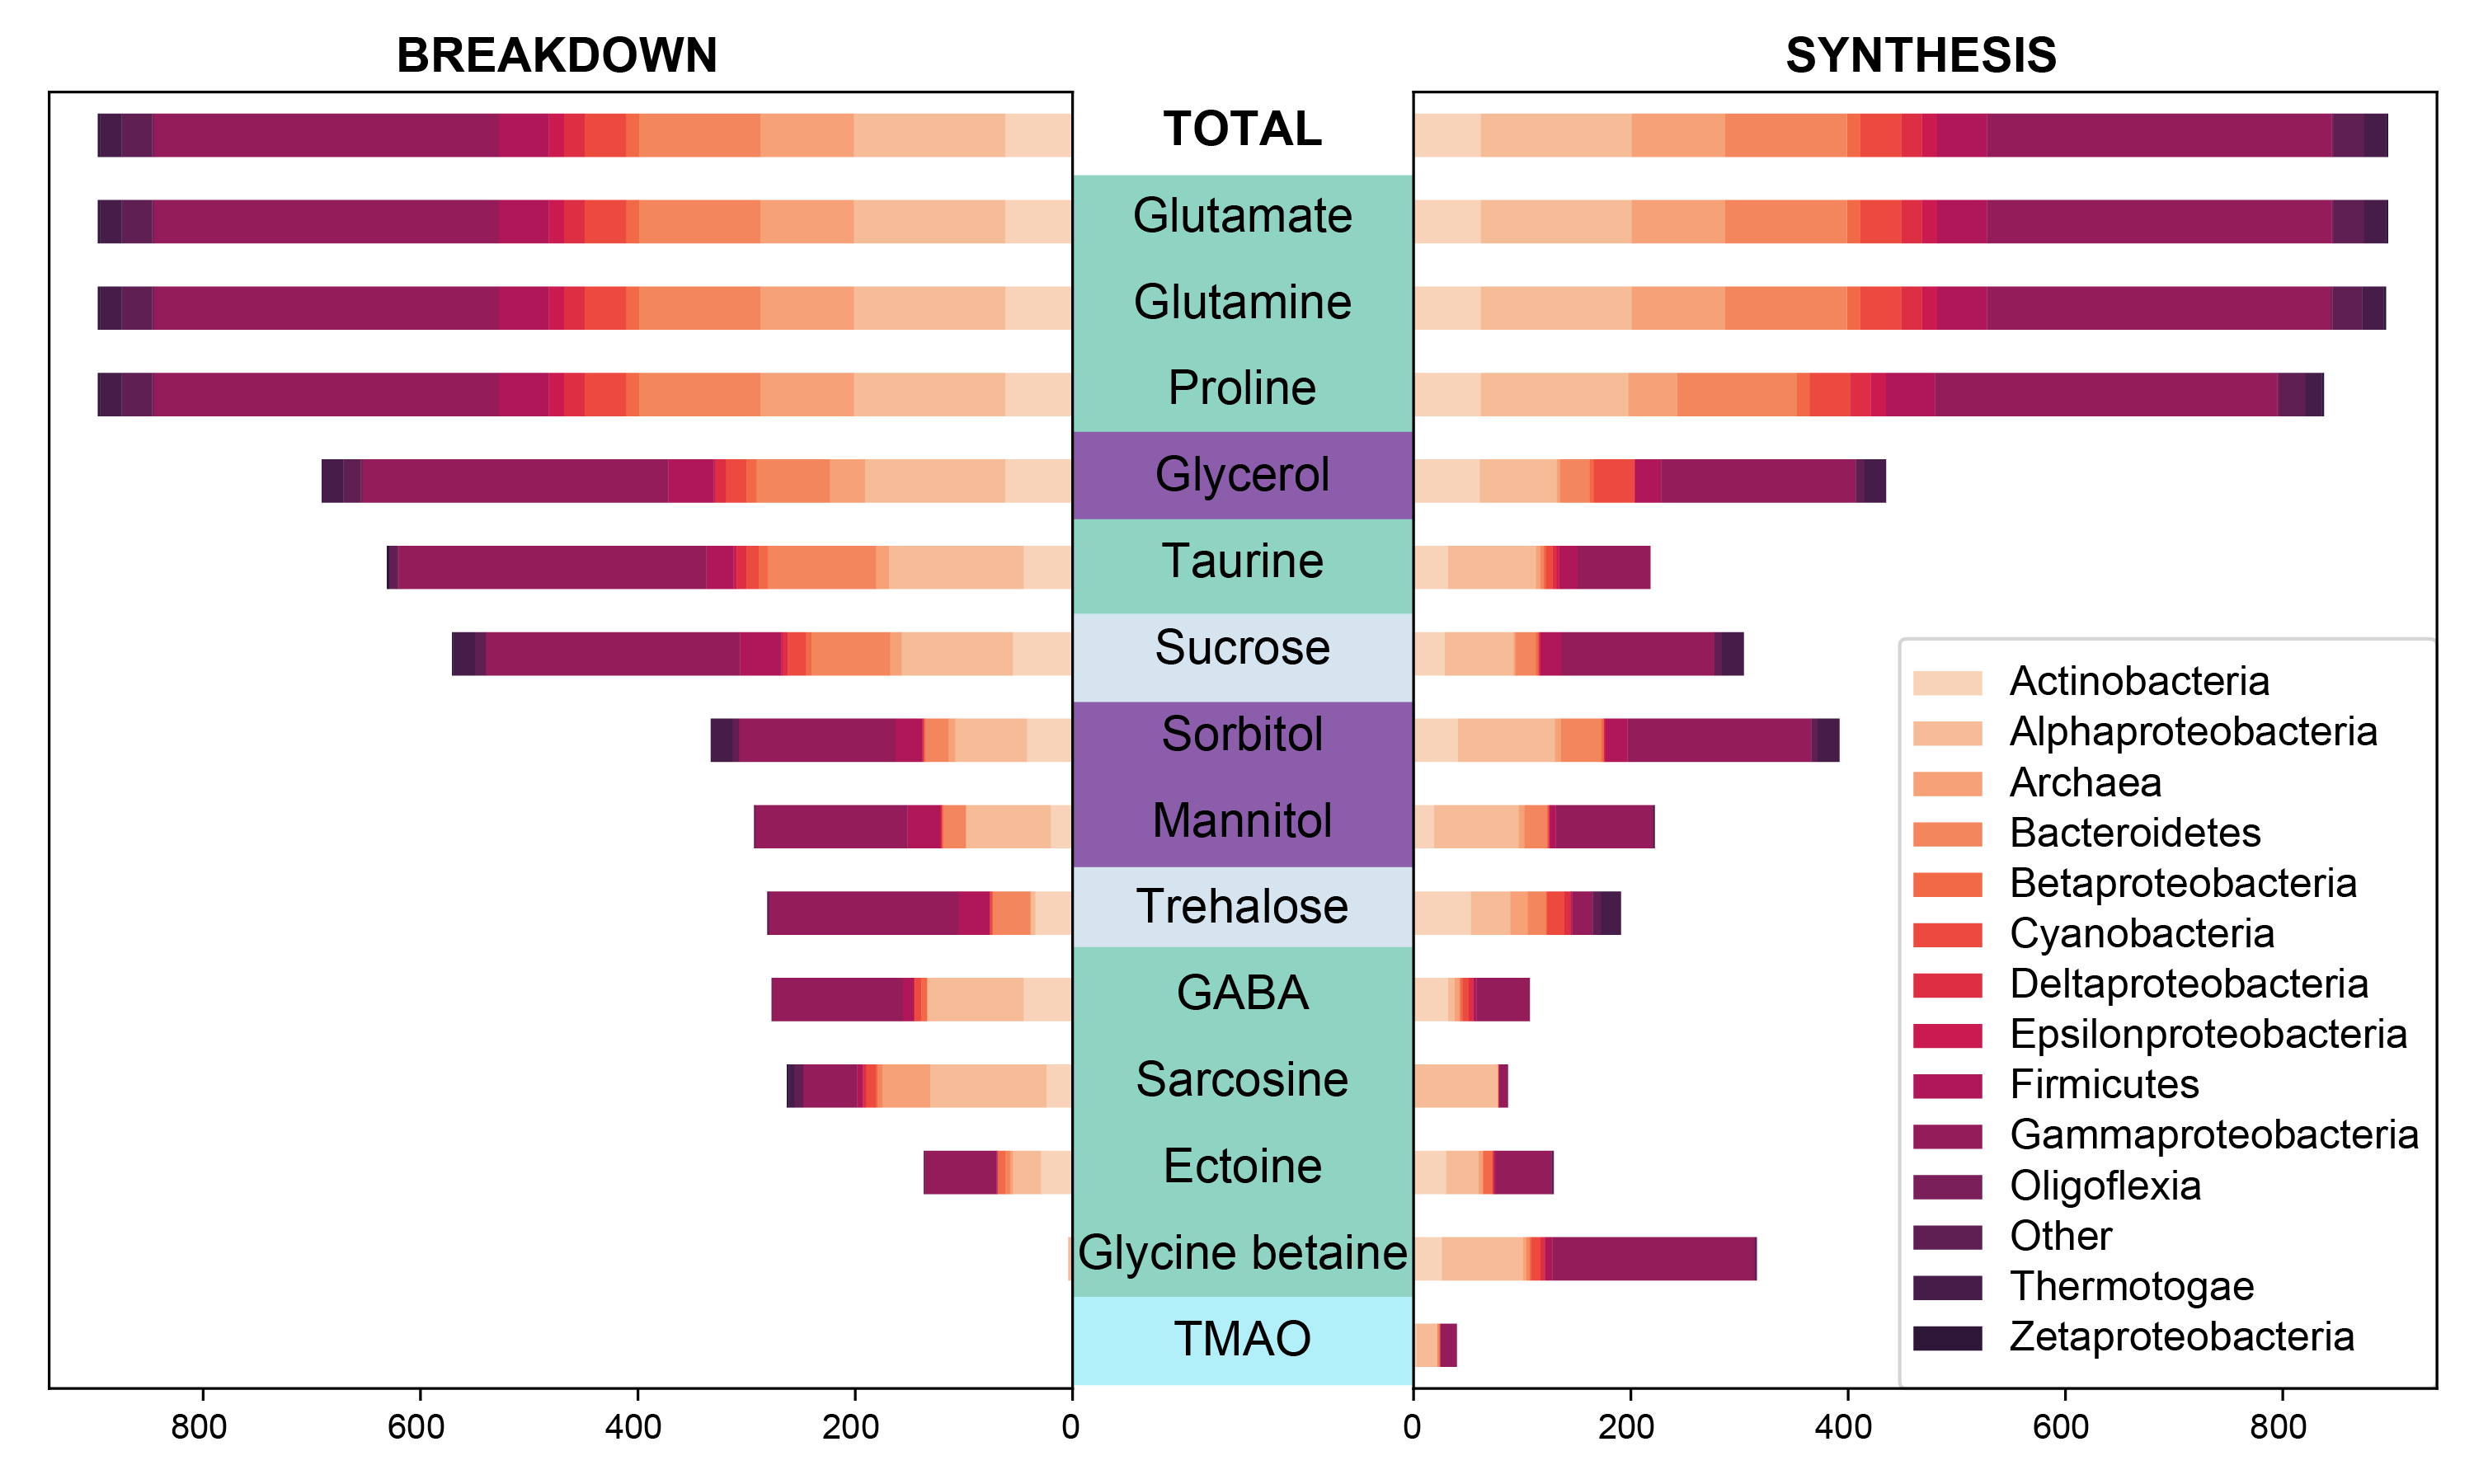
\includegraphics[width = 0.9\columnwidth]{Figures/Bacteria-Synthesis-Breakdown-v2021-03-14-01.png}
    \caption{The predicted synthesis and breakdown of targeted osmolytes across all (`Total`) MarRef bacterial and archaeal genomes (n = 897). The breakdown and synthesis of osmolytes is depicted as a stacked bar graph, and is colored by the designated taxonomic phylum (or class in the case of Proteobacteria). Osmolytes are colored by higher classification: amino acids and derivatives in green, sugar alcohols in purple, sugars in light periwinkle, and an amine oxide in cyan. Osmolytes are sorted along the y-axis based on the total number of genomes capable of breaking down a given osmolyte.}
    \label{fig:bact}
\end{figure}

We found that either: 1) breakdown and synthesis were tightly linked, suggesting core metabolism/internal recycling, or 2) breakdown and synthesis ability were unequal suggesting that the utilization of these osmolytes is a more specialized metabolism potentially only present in a smaller portion of the community. Additionally, most prokaryotic genomes that contained a transport system, also harbored the ability to synthesize and/or breakdown the respective osmolyte, except for glycine betaine for which many genomes were capable of transport without synthesis or breakdown.

\subsection{Amino acids and their derivatives}

\subsubsection*{Glutamate and Glutamine}
\begin{figure}[t!]
    \centering
    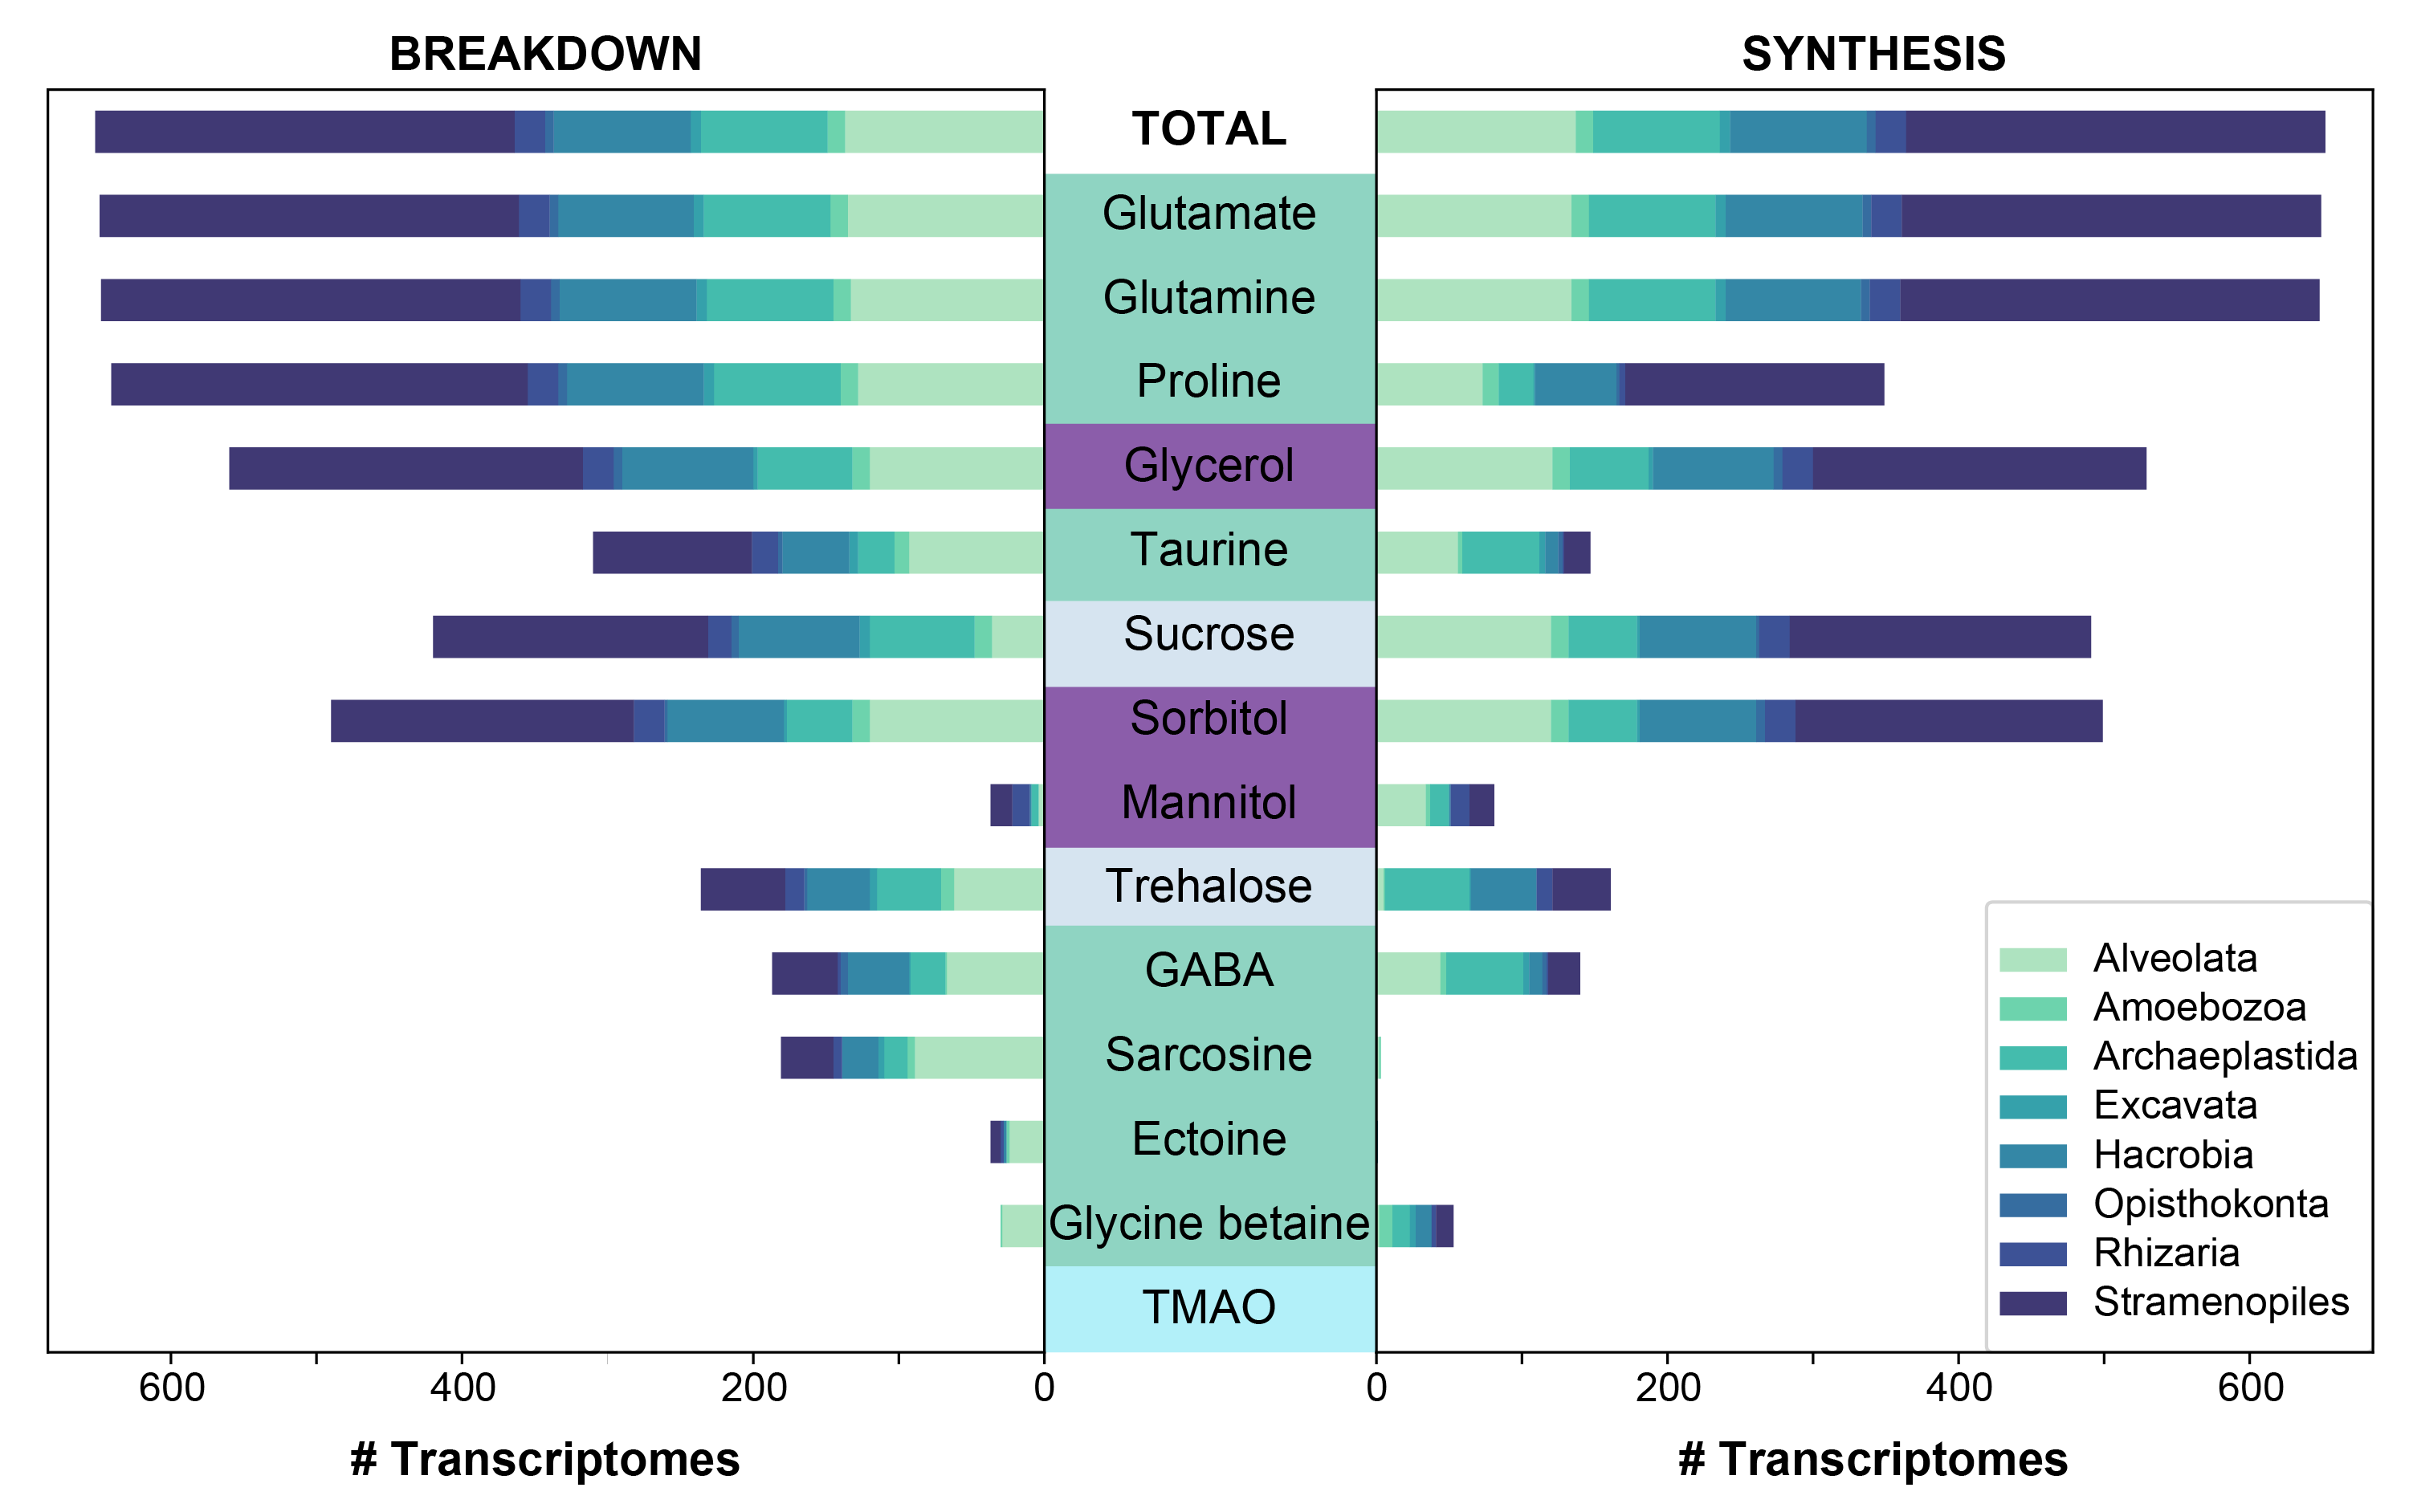
\includegraphics[width = 0.9\columnwidth]{Figures/Eukaryote-Synthesis-Breakdown-v2021-03-14-01.png}
    \caption{The predicted synthesis and breakdown of targeted osmolytes across all (`Total`) MMETSP protist transcriptomes (n = 652). The breakdown and synthesis of osmolytes is depicted as a stacked bar graph, and is colored by the designated taxonomic supergroup. Osmolytes are colored by higher classification: amino acids and derivatives in green, sugar alcohols in purple, sugars in light periwinkle, and an amine oxide in cyan. Osmolytes are sorted along the y-axis based on the total number of genomes capable of breaking down a given osmolyte for bacteria and archaea to be consistent with \Cref{fig:bact}.}
    \label{fig:euk}
\end{figure}
The ability to both synthesize and breakdown glutamate and glutamine was found in almost all prokaryotes (n = 897, n = 895, respectively) and eukaryotes (n = 647, n = 645, respectively) surveyed (\Cref{fig:euk-bac-comp}). This widespread function was expected as these amino acids play both a fundamental role in the creation and structure of proteins, and also in nitrogen recycling in cells \citep{Reitzer2003}. Additionally, glutamate and glutamine abundance has been documented to rapidly change in response to altered osmotic conditions \citep{Saum2008}. Only two prokaryotic genomes lacked the ability to synthesize glutamine, which was likely due to either an incomplete genome assembly or an issue of homology in our searches. The synthesis and breakdown of glutamate and glutamine was also missing in just 3 and 4 eukaryotic transcriptomes, respectively. Again, this was likely due to lack of coverage in the transcriptome, and potentially related to the physiological condition of the organism at the time of sequencing.

\subsubsection*{Proline}
Both breakdown and synthesis of proline was also common and widespread across prokaryotes (n = 838) and eukaryotes (n = 349), though slightly less so than glutamate and glutamine (\Cref{fig:euk-bac-comp}). In particular, Archaea (52\%) were less likely to have an identified proline synthesis pathway than bacterial groups (75-100\%) (\Cref{fig:bact}). Proline synthesis was much more variable across eukaryotic supergroups, ranging from 14-92\% (\Cref{fig:euk}). The observed trends for proline synthesis were similar to a previous study, which found that around 50\% of bacterial genomes had a complete proline synthesis pathway, and only 40\% and 30\% of archaeal and eukaryotic genomes, respectively, were capable of synthesis \citep{Mee2012}. 

As with glutamate and glutamine, proline fulfills an important role as an amino acid in proteins, but is also an osmolyte for bacteria \citep{Burg2008,Brill2011} and some marine diatoms \citep{Dawson2020,Dawson2020.2}, and can protect membranes from freezing \citep{Yancey2005}. More recently, proline was identified as the major organic osmolyte in the chemoautotroph \emph{Sulfurimonas} found around hydrothermal vents \citep{Gotz2018}. Interestingly, proline has been found to be abundant in deep sea particulate samples \citep{Takasu2015,Johnson2021} and in sinking marine particles \citep{Johnson2020}. One possible explanation for this could be increased use of proline as an osmolyte by organisms adapted to the colder temperatures of the deep ocean.
\begin{figure}[t!]
    \centering
    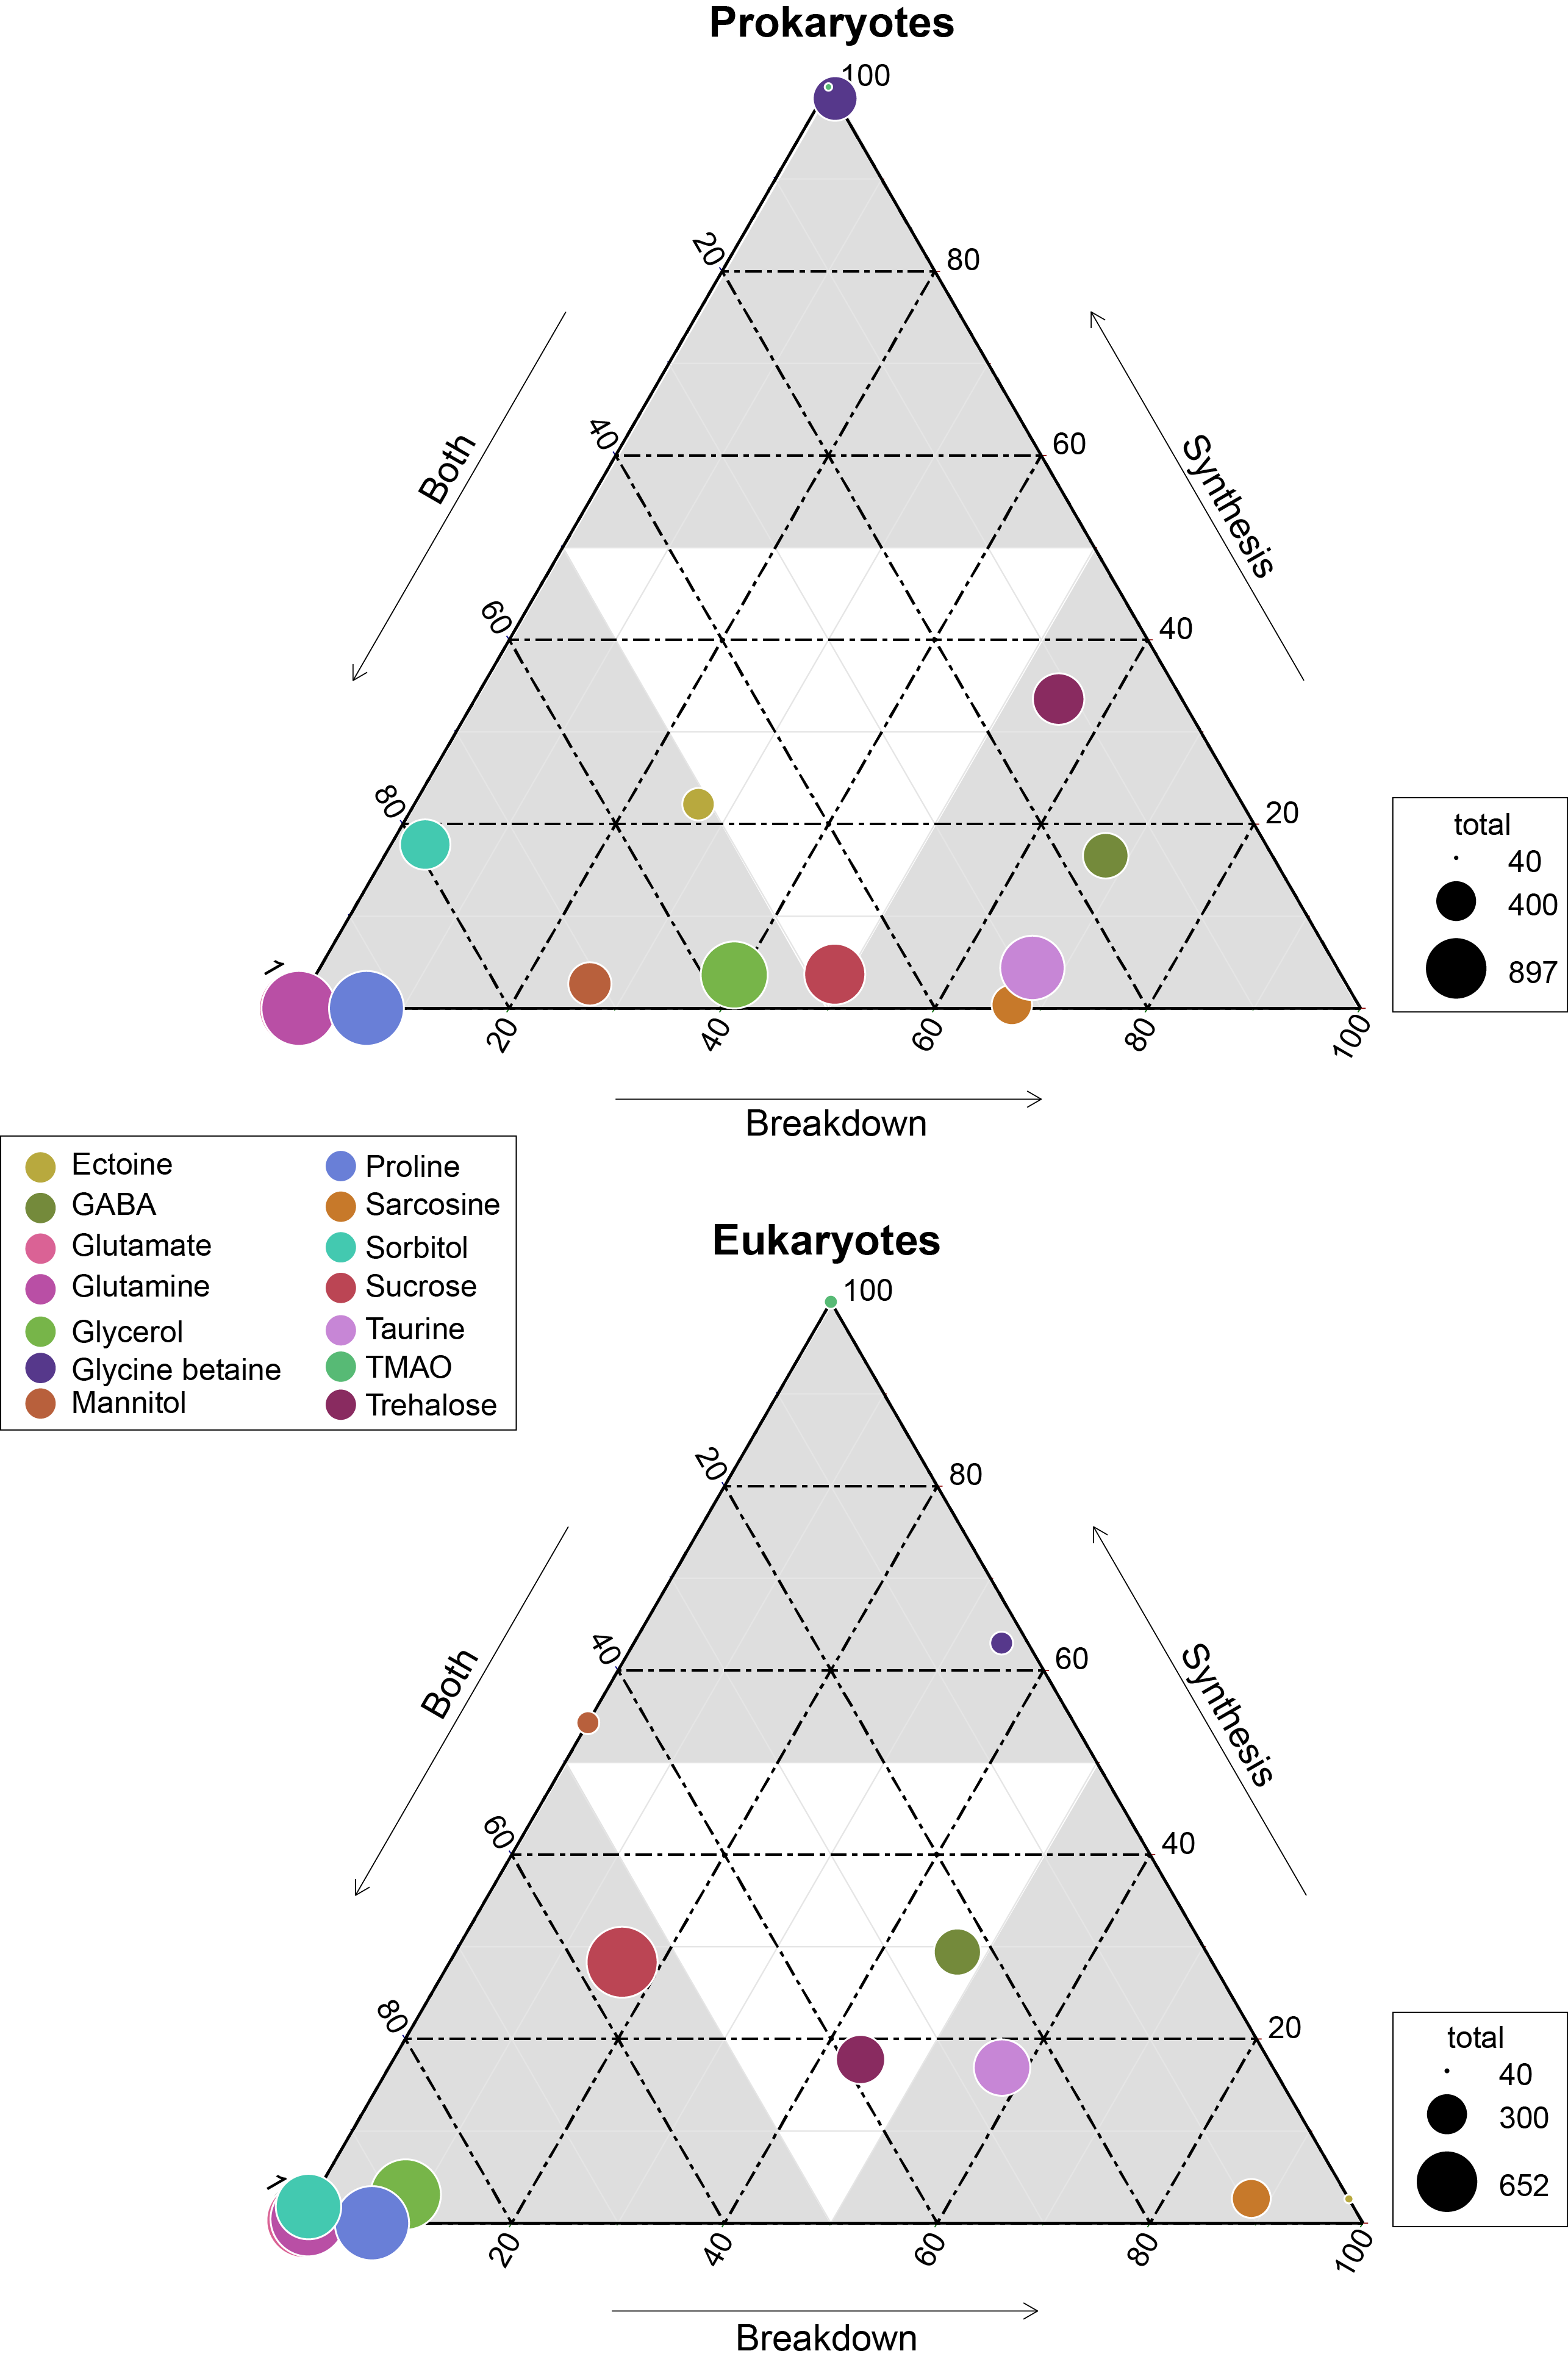
\includegraphics[width = 0.6\columnwidth]{Figures/ProkEukOverlapBW.png}
    \caption{Ternary plot of prokaryotes and eukaryotes osmolyte utilization based on genomic potential. Circle size represents total prokaryotes or eukaryotes capable of synthesis and/or breakdown of an osmolyte and circle placement represents the proportion of the total capable of synthesis, breakdown, or both synthesis and breakdown. Circle sizes are scaled by the total number of MarRef genomes (n = 897) and MMETSP transcriptomes (n = 652) surveyed. Osmolytes are designated by color as depicted in the legend. Glutamate is not clearly visible as it is found directly behind glutamine for both prokaryotes and eukaryotes.}
    \label{fig:euk-bac-comp}
\end{figure}
\subsubsection*{Taurine}
Broadly, the ability to synthesize taurine was less common than the ability to breakdown taurine across both prokaryotes and eukaryotes (\Cref{fig:euk-bac-comp}). A majority of prokaryotes were capable of taurine breakdown only (n = 442), and a smaller number were capable of both taurine breakdown and synthesis (n = 189) (\Cref{fig:euk-bac-comp}). Taurine synthesis was most common within Alphaproteobacteria (58\%) and Actinobacteria (52\%) (\Cref{fig:bact}). The breakdown of taurine in typically heterotrophic bacteria (i.e. Proteobacteria, Firmicutes, Bacteroidetes) ranged from 21\% to 100\% (\Cref{fig:bact}). Breakdown and synthesis of taurine was limited in Cyanobacteria (29\% breakdown and 16\% synthesis). These findings are consistent with previous work that identified bacterial uptake of taurine by three Proteobacteria groups: SAR11, Roseobacter, and \emph{Alteromonas}, and also Thaumarchaeota and Euryarchaeota \citep{Clifford2020,Clifford2019}. Metaproteomic data from the Ross Sea also indicated that SAR11 was a significant taurine sink via uptake and degradation \citep{Williams2012}. Prokaryotes capable of taurine transport (n = 53) were almost exclusively limited to Proteobacteria and were all also capable of taurine synthesis and/or breakdown (\Cref{fig:transporters}). 

Taurine synthesis and breakdown was overall less common across eukaryotes (\Cref{fig:euk} \& \ref{fig:euk-bac-comp}). As observed for prokaryotes, the ability to only breakdown taurine was also most common in eukaryotes surveyed (n = 226) (\Cref{fig:euk-bac-comp}). Taurine synthesis was most common in Archaeplastida (61\%) (\Cref{fig:euk}). Interestingly, Archaeplastida were far less likely to be capable of taurine breakdown (29\%). This contrasts with the other eukaryotic supergroups which had limited synthesis (e.g. Stramenopiles (6\%), Hacrobia, (10\%), and Alveolata (41\%)) and greater potential for breakdown (38\%, 49\%, and 68\%, respectively) (\Cref{fig:euk}). Dissolved taurine concentrations in the Gulf of Alaska and the North Atlantic indicate that concentrations are typically in the low nanomolar range, and that release by amphipod-copepod assemblages in the Pacific occurs at rates of around 0.8 µmol g\textsuperscript{-1} C-biomass hr\textsuperscript{-1} and from Atlantic copepods at rates ranging from 1.3-9.5 $\mu$mol g\textsuperscript{-1} C-biomass hr\textsuperscript{-1} \citep{Clifford2017}. In the Adriatic Sea, even higher rates of release were found in mixed mesozooplankton communities, reaching the highest rates in the fall of an average of 59 $\mu$mol g\textsuperscript{-1} C-biomass hr\textsuperscript{-1} \citep{Clifford2020}. While our results indicate that protists are potential taurine sinks, zooplankton, specifically copepods, are clearly important taurine sources in the microbial loop. Multicellular eukaryotes (not represented in MMETSP) should be considered with respect to taurine recycling in the oceans, and possibly in addition to some other marine eukaryotes (mussels and tubeworms) that use taurine \citep{Yin2000,Hosoi2005}.


\subsubsection*{Glycine Betaine}
Glycine betaine synthesis was more common than breakdown in both prokaryotes and eukaryotes (\Cref{fig:euk-bac-comp}). Most prokaryotes were only capable of glycine betaine synthesis (n = 316) (\Cref{fig:euk-bac-comp}). In particular, a majority of Alphaproteobacteria (54\%) and Gammaproteobacteria (59\%) were capable of synthesis. The ability to breakdown glycine betaine was extremely rare across prokaryotes (\Cref{fig:bact}). The small number of prokaryotes capable of breakdown (n = 4) were not able to synthesize glycine betaine (\Cref{fig:euk-bac-comp}) and were exclusively observed in Alphaproteobacteria strains: Candidatus \emph{Pelagibacter ubique}, Alphaproteobacterium HIMB5, Alphaproteobacterium HIMB59, and \emph{Rhodovulum sulfidophilum}. Glycine betaine synthesis and breakdown was also rare in Archaea, where only 4\% were capable of synthesis and no Archaea were capable of breakdown. The ability to breakdown glycine betaine by bacteria is clearly a highly specialized metabolic ability. Interestingly, the majority of prokaryotes capable of glycine betaine transport cannot breakdown or synthesize (n = 190) or can only synthesize glycine betaine (n = 234)  (\Cref{fig:transporters}). This stands in stark contrast to our observations of taurine transporter co-occurrence with synthesis and/or breakdown, where no genomes contained only a taurine transporter (\Cref{fig:transporters}). In addition, transport of glycine betaine was found more frequently than for other osmolytes, and the presence of the two different glycine betaine transporters was taxa dependent. Proteobacteria primarily have the osmoprotectant ABC transporter, whereas Actinobacteria primarily have the glycine betaine/proline ABC transporter. A majority of Firmicutes contained both the osmoprotectant and the glycine betaine/proline ABC transporters, and notably did not contain any other osmolyte transporters (\Cref{fig:transporters}). The widespread ability for glycine betaine transport without breakdown suggests that this osmolyte is likely targeted by bacteria for cellular retention to function as an osmolyte, which was observed previously by direct measurements of radiolabeled glycine betaine uptake \citep{Kiene1998}. Glycine betaine was the only osmolyte in our survey that appeared to be targeted for osmotic function by bacteria, rather than as a carbon and/or nitrogen substrate to be metabolized. 

Glycine betaine synthesis and breakdown was also limited in eukaryotes (\Cref{fig:euk}), and the majority were only capable of synthesis (n = 53) (\Cref{fig:euk-bac-comp}). Notably, glycine betaine synthesis was most common in Amoebozoa (75\%) and Excavata (57\%), while in other groups, synthesis was $< 14\%$ prevalent (\Cref{fig:euk}). The breakdown of glycine betaine was absent from all groups except for Alveolata (21\%) and Amoebozoa (8\%) (\Cref{fig:euk}). Glycine betaine was previously measured in monocultures of Hacrobia (\textit{Chrysochromulina sp.}, \textit{Emiliania huxleyi}) and Alveolata (\textit{Amphidinium carteraea}, \textit{Prorocentrum minimum}), and some diatoms (\textit{Thalassiosira pseudonana}) \citep{Gebser2013,Keller1999,Keller1999.2}. These direct measurements of cellular osmolytes suggest we under-predicted glycine betaine synthesis in our analysis. It is possible however that glycine betaine synthesis was not upregulated in the conditions the reference transcriptomes were collected in. 

\subsubsection*{Sarcosine}
Sarcosine is structurally very similar to glycine betaine, but it lacks two methyl groups relative to glycine betaine. Sarcosine breakdown was much more common in both prokaryotes and eukaryotes (\Cref{fig:euk-bac-comp}). Sarcosine synthesis was not present in prokaryotes, except Alphaproteobacteria of which 55\% contained a synthesis pathway (\Cref{fig:bact}). Relative to synthesis, sarcosine breakdown was far more common across prokaryotic groups, particularly in Actinobacteria, Archaea, and Alphaproteobacteria (39\%, 51\%, 77\%, respectively). Sarcosine synthesis was almost completely absent in all eukaryotes (\Cref{fig:euk}). As observed for prokaryotes, more eukaryotes were capable of sarcosine breakdown, including most Amoebozoa, Excavata, and Alveolata (42\%, 57\%, 65\%, respectively). While sarcosine as an osmolyte in marine organisms does not seem to have been extensively studied, elasmobranchs have been shown to use sarcosine to counteract increased levels of urea \citep{Treberg2006}, and, generally, for decades, sarcosine has been considered to act as an osmolyte \citep{Arakawa1985}. Sarcosine can be synthesized from creatine, choline, or glycine (Supplemental Data Sheet 1). As the ability to synthesize sarcosine was mostly absent in prokaryotic and eukaryotic groups, except in Alphaproteobacteria, it suggests that the source of sarcosine in the ocean is relatively unknown. However, sarcosine is an intermediary product formed during the breakdown of glycine betaine (glycine betaine \textrightarrow dimethylglycine \textrightarrow  sarcosine \textrightarrow glycine) (Supplemental Data Sheet 1), and therefore the incomplete breakdown of glycine betaine could be a possible source of sarcosine in the ocean.

\subsubsection*{Ectoine}
Ectoine metabolism was less widely distributed across prokaryotes and eukaryotes compared to the other osmolytes (\Cref{fig:bact} \& \ref{fig:euk}). Within the small number of prokaryotes with ectoine metabolism, most were capable of both synthesis and breakdown (n = 90), while a smaller number were only capable of breakdown (n = 47) or only capable of synthesis (n = 39) (\Cref{fig:euk-bac-comp}). Ectoine synthesis and breakdown had a fairly similar taxonomic distribution within prokaryotes. For example, $\sim 48\%$ of Actinobacteria and $\sim20\%$ of Alphaproteobacteria were capable of both synthesis and breakdown (\Cref{fig:bact}). However, the Betaproteobacteria (n = 12 genomes in MarRef) had the highest proportion of synthesis (75\%) and breakdown (58\%). Notably, ectoine synthesis and breakdown pathways were completely absent in Cyanobacteria, and were very rare in Archaea (5\% synthesis, 2\% breakdown). Ectoine is known to be an important osmolyte for \emph{Halomonas} sp. \citep{Ono1999} and has also been found to be used across species of \emph{Vibrio}, both those that are associated with other organisms, like fish or shellfish, or planktonic species \citep{Pflughoeft2003,Ongagna-Yhombi2013,Ma2017}. Ectoine synthesis was completely absent in eukaryotes, except for one Hacrobia strain, which was likely a result of prokaryotic contamination of the transcriptome (\Cref{fig:euk}). A very small number of eukaryotes were capable of ectoine breakdown ($< 18\%$ in all supergroups). Ectoine is typically considered to be a prokaryotic osmolyte, but was recently observed in Stramenopiles (n = 2 diatoms), Hacrobia (n = 2 haptophytes, n = 1 coccolithophore), and Alveolata (n = 1 dinoflagellate) \citep{Fenizia2020}. Specifically, the diatoms were shown to take-up ectoine in xenic cultures, and also synthesize ectoine in axenic monocultures, but only one of the three genes used by bacteria for ectoine synthesis had a putative homolog in the genome of the diatom \emph{Phaeodactylum tricornutum} \citep{Fenizia2020}. This low homology with bacterial ectoine synthesis genes may explain why we also did not find significant ectoine synthesis in the eukaryotic transcriptomes surveyed here.

\subsubsection*{GABA}
The synthesis and breakdown of Gamma-aminobutyric acid (GABA) was also found to be relatively rare compared to other osmolytes in both prokaryotes and eukaryotes (\Cref{fig:euk-bac-comp}). Most prokaryotes were only capable of GABA breakdown (n = 225), compared to a smaller number capable of synthesis only (n = 55), or both synthesis and breakdown (n = 52) (\Cref{fig:euk-bac-comp}). A majority of Actinobacteria (73\%) and Alphaproteobacteria (63\%) were capable of GABA breakdown (\Cref{fig:bact}). GABA synthesis was also common in Actinobacteria (52\%), but less so in other groups (e.g. Alphaproteobacteria 4\%). The ability to only breakdown GABA was most common in eukaryotes (n = 125) (\Cref{fig:euk-bac-comp}), but some proportion of every supergroup was capable of GABA synthesis or breakdown, ranging from 5\% - 61\% synthesis and 8\% - 83\% breakdown across supergroups (\Cref{fig:euk}). In particular, a large portion of Archaeplastida were capable of synthesis (57\%), but breakdown was relatively constrained (27\%). GABA has been identified in certain species of marine yeast at much higher concentrations than commercial yeast \citep{Masuda2008}, and is an indicator of ecosystem health in snapper \citep{Goode2020}. In marine bacteria, greater quantities of GABA are released from cells in response to decreased sodium chloride concentrations or increased pH \citep{Mountfort1992}. GABA is also used as a settlement queue for marine invertebrates, however, around 1/3 of bacteria isolated from a potential settlement site were also found to metabolize GABA and have high- and low-affinity transporters for the substrate \citep{Kaspar1991}. This suggests a complex role in marine environments where GABA serves as a signaling compound, osmolyte, and carbon substrate.

\subsection{Amine oxide}

\subsubsection*{TMAO}
Only one pathway for synthesis and breakdown of TMAO was identified within the KEGG framework (\Cref{tabl:pathnum}), which limited our analysis of TMAO synthesis, breakdown, and transport as more pathways likely exist. We identified synthesis pathways for trimethylamine N-oxide (TMAO) in a few prokaryotic groups: Actinobacteria (5\%), Alphaproteobacteria (14\%), Bacteroidetes (2\%), Cyanobacteria (3\%), and Gammaproteobacteria (5\%). However, this is likely due to limitations of the pathways annotated in KEGG. TMAO is found in deep sea animals including teleosts, skates, and crustaceans where it is thought to play an additional role as a protectant from the high hydrostatic pressure of the deep ocean \citep{Yancey2002}. Nanomolar concentrations of TMAO have been measured in Antarctic surface waters as well, indicating a role throughout the water column \citep{Gibb2004}, and copepods have been shown to produce TMAO from trimethylamine \citep{Strom1979}.

\subsection{Sugars and sugar alcohols}

\subsubsection*{Sorbitol}
Both the breakdown and synthesis of sorbitol were equally distributed in prokaryotes and eukaryotes, though a larger percentage of eukaryotes had the ability to breakdown and synthesize sorbitol (\Cref{fig:euk-bac-comp}). More than 40\% of all Actinobacteria, Firmicutes, Alphaproteobacteria, and Gammaproteobacteria were capable of sorbitol breakdown and synthesis (\Cref{fig:bact}). Cyanobacteria appeared to be missing all of the single step pathways for sorbitol breakdown and sorbitol synthesis (\Cref{tabl:pathnum} \& \Cref{fig:bact}). Sorbitol synthesis by prokaryotes was more common than expected as prokaryotes typically do not use polyols (e.g. sorbitol and mannitol) as compatible solutes \citep{Kinne1993,Empadinhas2008}. Both sorbose and sorbitol were previously identified as metabolites that are rapidly consumed from the dissolved pool \citep{Vorobev2018}. Here, the breakdown of sorbose to sorbitol was annotated as a sorbitol synthesis pathway, and therefore it is possible that many of the prokaryotes identified to be capable of sorbitol synthesis actually utilize this pathway to breakdown sorbose. Additionally, the majority of prokaryotes that were capable of sorbitol transport (n = 100) also contained sorbitol breakdown and synthesis pathways (\Cref{fig:transporters}). Only a small number of prokaryotes (n = 7) contained all subunits of the sorbitol/mannitol transporter without the ability to synthesize or breakdown sorbitol.  Sorbitol synthesis and breakdown was broadly and commonly distributed across the eukaryotic supergroups surveyed (\Cref{fig:euk}). An average $\sim 70\%$ of each eukaryotic group was also capable of sorbitol breakdown and/or synthesis, except for the Excavata (\Cref{fig:euk}). The widespread ability to synthesize and breakdown sorbitol in eukaryotes was expected as polyols have previously been observed to function as compatible solutes in eukaryotes \citep{Burg2008}, and sorbitol has been observed to increase with salinity in microalgae \citep{Brown1978}. 

\begin{figure}[b!]
    \centering
    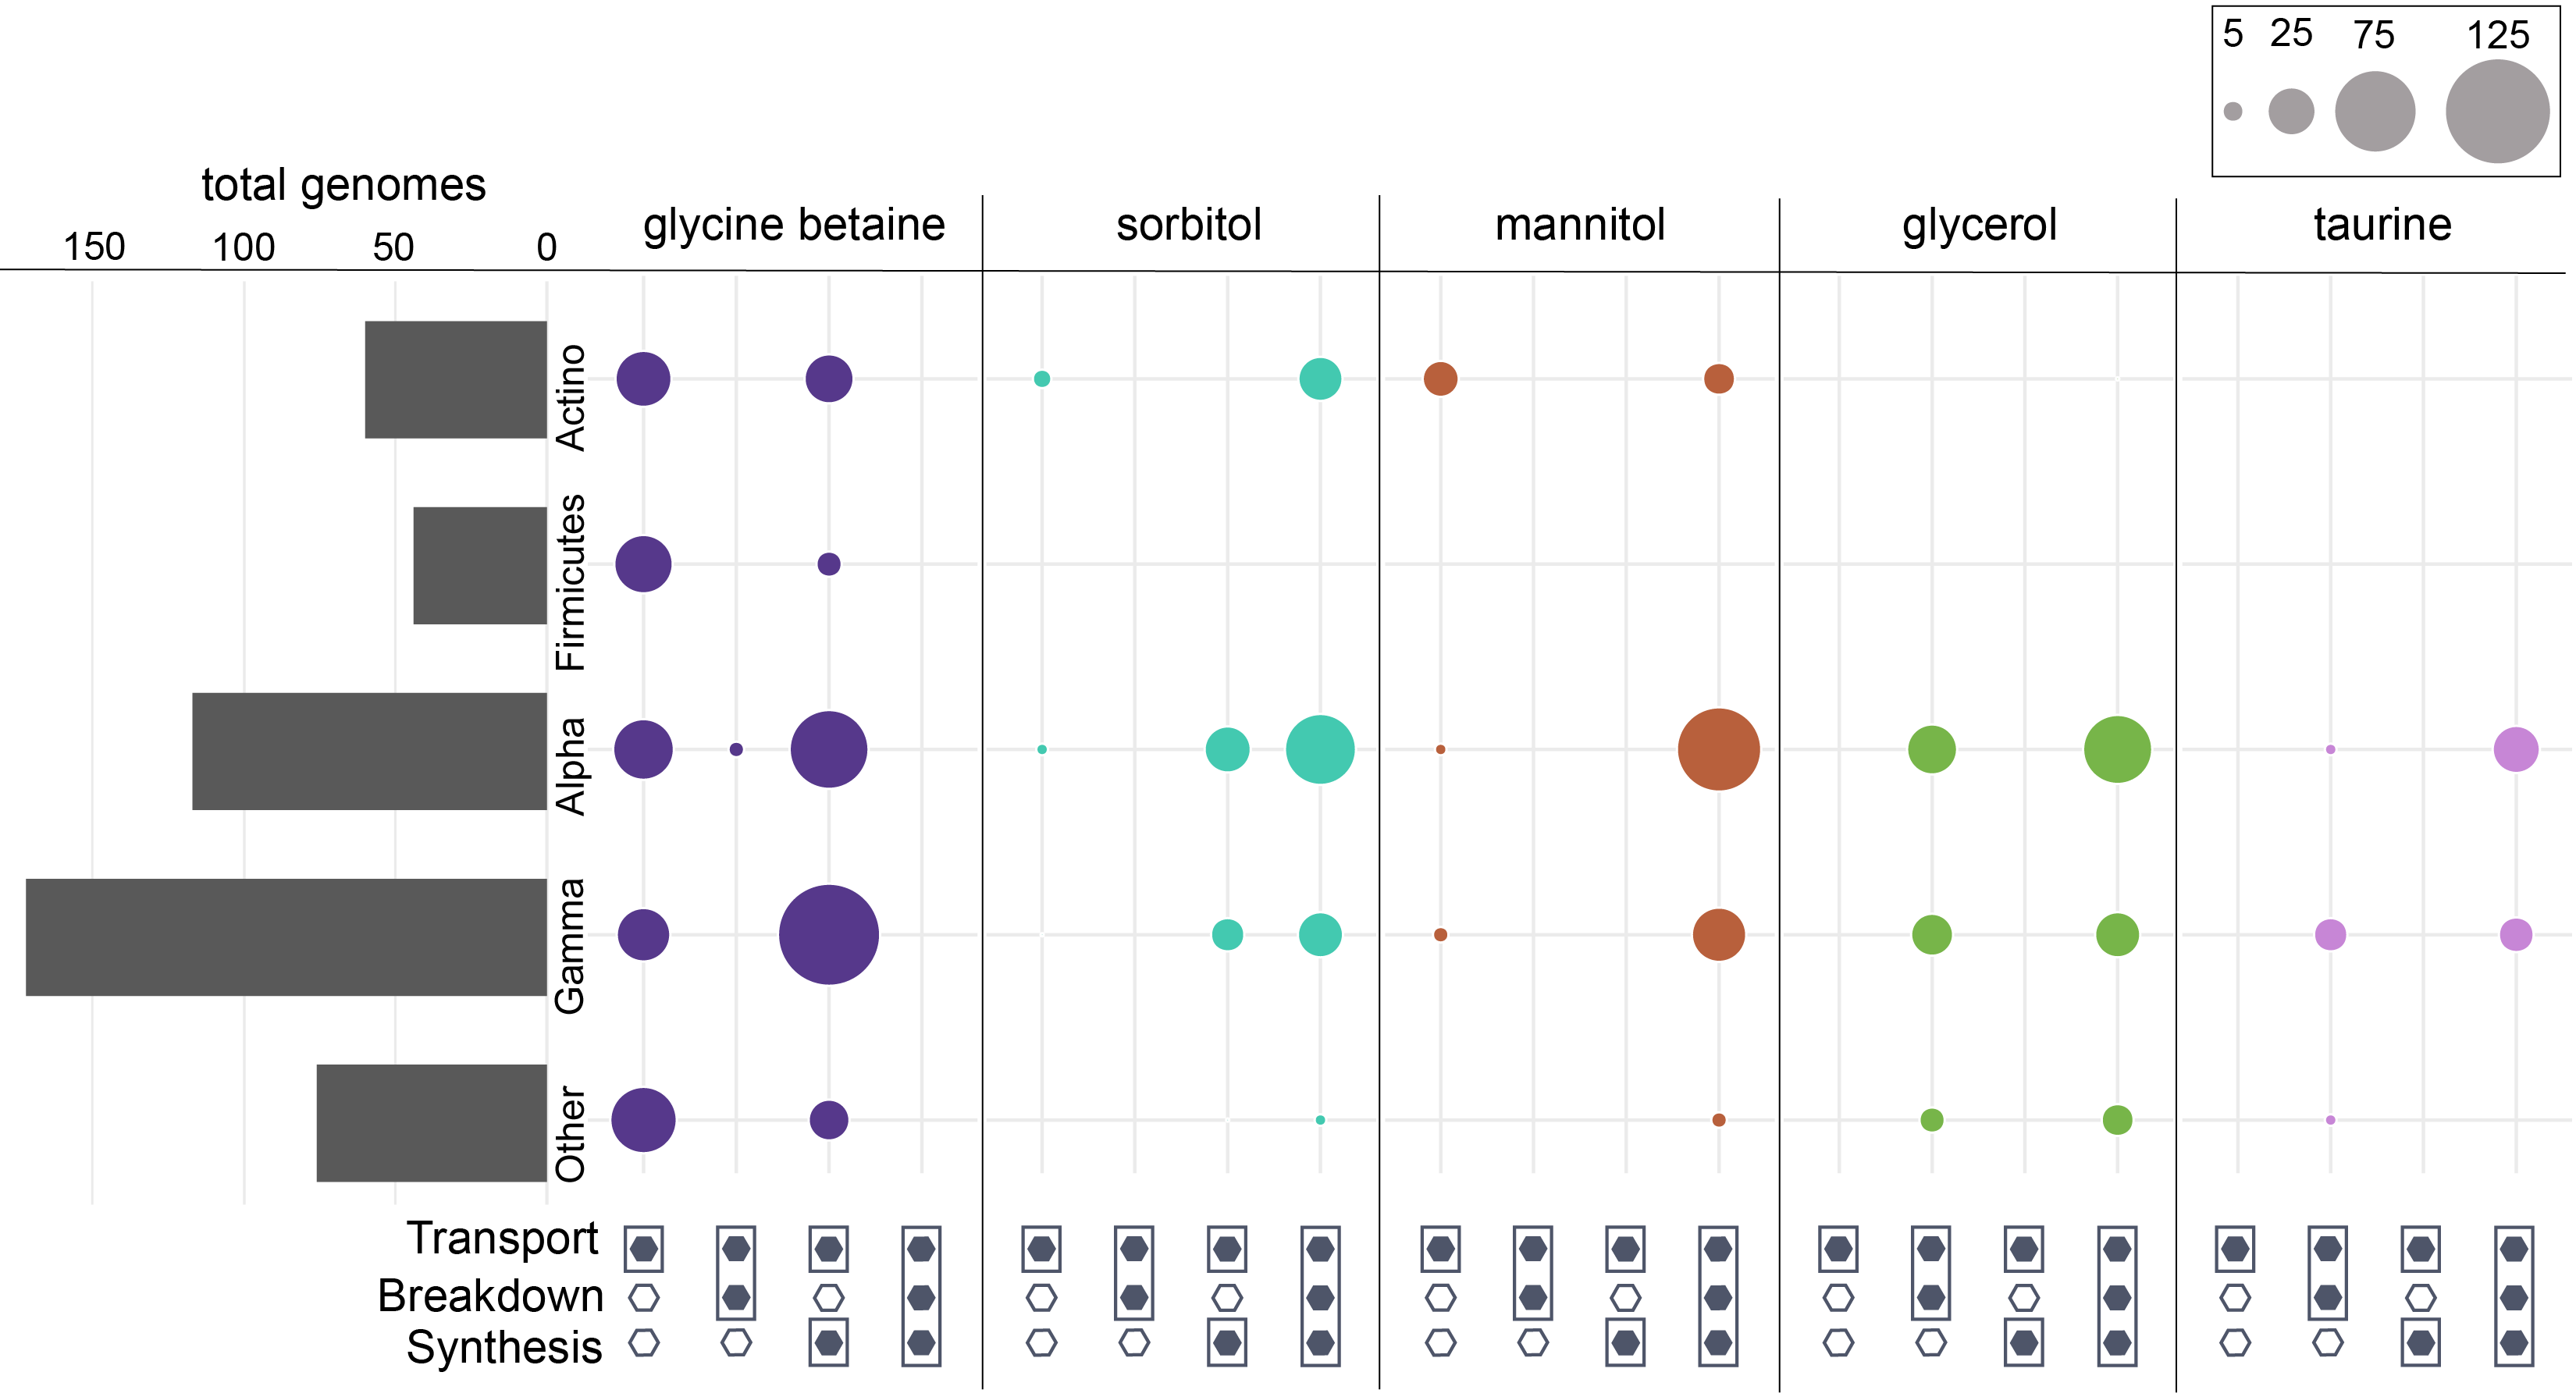
\includegraphics[width = 0.9\columnwidth]{Figures/transportersummary.png}
    \caption{Prokaryotic genomes that contained one or more of the osmolyte ABC transporters annotated in KEGG. Bars represent the total number of genomes that contained at least one transporter. 'Other' represents taxa that contributed $<10\%$ of the total. For each respective osmolyte, circles represent the total number of genomes in each group that were capable of transport only, transport and breakdown, transport and synthesis, or all (transport, breakdown, and synthesis). Missing circles indicate no genomes with the respective category.  }
    \label{fig:transporters}
\end{figure}

\subsubsection*{Mannitol}
Mannitol breakdown and synthesis was less common in both prokaryotes and eukaryotes (\Cref{fig:euk-bac-comp}). Mannitol synthesis and breakdown was broadly found across all Proteobacteria ($< 60\%$) and Actinobacteria ($\sim 30\%$), whereas more Firmicutes had the potential to breakdown mannitol (65\%) compared to synthesis (11\%) (\Cref{fig:bact}). Mannitol was also not expected to be widespread across prokaryotes as polyols are uncommon in prokaryotes \citep{Empadinhas2008}, and mannitol synthesis has been previously observed in prokaryotes but in a limited number of taxa. Specifically, a soil Gammaproteobacterium synthesized mannitol \emph{de novo} when other osmolyte sources were not provided exogenously \citep{Sand2013}. As observed for sorbitol, few prokaryotes (n = 26) were capable of sorbitol/mannitol transport only, and the majority of prokaryotes capable of mannitol transport were also able to both synthesize and breakdown mannitol (n = 124) (\Cref{fig:transporters}). The presence of the transporter alongside breakdown and synthesis pathways suggests that 1) sorbitol and mannitol are not transported for osmotic function only, and 2) the transporter may actually be important for efflux with respect to internal recycling of the osmolytes. Mannitol utilization was even less common in eukaryotes (\Cref{fig:euk}). Eukaryotic synthesis and breakdown of mannitol was most common in Rhizaria ($> 50\%$), but not common in their potential Hacrobia symbiotic partners (1\%). Mannitol was previously found to be present in Archaeplastida \citep{Kirst1989}, and was shown to increase with salinity in three Archaeplastida strains of Chlorophytes \citep{Dickson1987.2}. Relative to Rhizaria though, mannitol synthesis was limited in Archaeplastida (only 15\%), though this supergroup encompasses a large diversity of eukaryotes.

\subsubsection*{Glycerol}
Glycerol synthesis and breakdown was common across prokaryotes and eukaryotes, but the presence of breakdown and synthesis was not even in prokaryotes (\Cref{fig:euk-bac-comp}). While Actinobacteria were almost equally capable of synthesis (98\%) and breakdown (100\%), Proteobacteria were 2-fold more capable of breakdown (93\%) than synthesis (51\%) (\Cref{fig:bact}). In contrast, Cyanobacteria were 2-fold more capable of synthesis (92\%) than breakdown (50\%). Globally, 31\% of prokaryotes were only capable of glycerol breakdown, lacking the ability to synthesize (\Cref{fig:euk-bac-comp}). Prokaryotes that can transport glycerol (n = 139) were almost exclusively limited to Proteobacteria and are all capable of synthesis and/or breakdown of glycerol (\Cref{fig:transporters}). In eukaryotes, 78\% were capable of both synthesis and breakdown of glycerol, with the ability broadly spread across groups (\Cref{fig:euk} \& \ref{fig:euk-bac-comp}). Glycerol is one of the major byproducts of photosynthesis that is often released and shared within algal-host symbioses and has also been found to be induced under osmotic stress in model symbiotic algae such as \emph{Symbiodinium} \citep{Suesc_n_Bol_var_2016, Mayfield_2007}. Moreover, glycerol has been found to increase the activity and abundance of mixotroph-associated bacteria (e.g. Alphaproteobacteria and Gammaproteobacteria), and may act as a key currency of exchange between protists and prokaryotes in the marine system \citep{Poddar_2018}.  

\subsubsection*{Sucrose}
The breakdown of sucrose was at least 2-fold more common than the synthesis of sucrose in all prokaryotic groups, except for Thermotogae (\Cref{fig:euk-bac-comp}). All of the references in the Thermotogae group surveyed in MarRef (n = 20) are capable of both synthesis and breakdown of sucrose. This group includes known hyperthermophilic chemoorganotrophic organisms such as \emph{Thermotoga maritima}, which are known to metabolize many simple and complex carbohydrates \citep{NELSON2001169}. The general bias towards sucrose breakdown may suggest that prokaryotes primarily rely on other organisms for sucrose supply. Although sucrose has been shown to serve an osmotic function in Cyanobacteria and other photosynthetic organisms \citep{Reed1986,Klahn2011}, the sucrose synthesis pathway was unexpectedly incomplete based on our three-step definition (Supplemental Data Sheet 1) in Cyanobacteria genomes surveyed in MarRef (n = 38), which included \emph{Synechococcus}, \emph{Prochlorococcus}, known nitrogen fixers, and others. All Cyanobacteria genomes were missing the pathway's first step (conversion of glucose-1-phosphate to UDP-glucose). The majority of \emph{Synechococcus} and \emph{Prochlorococcus} genomes contained the glucosyltransferase required for the second step (conversion of UDP-glucose to sucrose-6-phosphate), but not the phosphatase required for the third step (sucrose-6-phosphate hydrolysis). The few other Cyanobacteria (\emph{Calothrix} and \emph{Nodularia}) (n = 9) did contain the phosphatase for the third step but were missing the enzymes for the first two steps. Sucrose utilization was common in eukaryotes (n = 586), and the majority were capable of both synthesis and breakdown (\Cref{fig:euk-bac-comp}). Amoebozoa, Hacrobia, Rhizaria, and Stramenopiles were all most frequently capable of both synthesis and breakdown (\Cref{fig:euk}). In contrast, Alveolata had 3-fold more synthesis pathways than breakdown, suggesting that sucrose may potentially be a  significant osmolyte for dinoflagellates. 

\subsubsection*{Trehalose}
The breakdown and synthesis of trehalose exhibited unique trends across the major prokaryotic groups surveyed, where either only synthesis or only breakdown were more common than the ability to both synthesize and breakdown (\Cref{fig:bact} \& \ref{fig:euk-bac-comp}). This suggests that trehalose is less likely to be internally recycled, but rather it is either synthesized as an osmolyte, or consumed as a carbon source. Trehalose synthesis was more common in Actinobacteria (86\%), Alphaproteobacteria (26\%), Archaea (19\%), and Cyanobacteria (42\%), whereas trehalose breakdown was more common in Bacteriodetes (30\%), Firmicutes (63\%), and Gammaproteobacteria (55\%) (\Cref{fig:bact}). Interestingly, 90\% of Thermotogae surveyed were capable of trehalose synthesis, but no trehalose breakdown. Trehalose was found to be a primary osmolyte in \emph{Crocosphaera watsonii}, instead of glucosylglycerol which is typically used by marine Cyanobacteria \citep{Pade2012}. Many non-marine bacteria use this osmolyte, suggesting that this capability in \emph{Crocosphaera} may have been obtained through horizontal gene transfer \citep{Pade2012}. A new trehalose synthase gene that converts maltose to trehalose has also been identified in a marine species of \emph{Pseudomonas} \citep{Gao2013}. Intracellular concentrations of trehalose have been found to fluctuate on a diel cycle in the north Pacific subtropical gyre \citep{Boysen2020}, suggesting that it might be important in the physiology of oligotrophic bacteria, such as nitrogen fixers. Trehalose breakdown relative to trehalose synthesis was at least 5-fold more common in the potentially mixotrophic or heterotrophic eukaryotic groups of Alveolata (43\%), Amoebozoa (75\%), and Excavata (71\%) . The other eukaryotic groups (Archaeplastida, Hacrobia, and Stramenopiles) were more often capable of both breakdown and synthesis (\Cref{fig:euk} \& \ref{fig:euk-bac-comp}). Trehalose has been found to be abundant and to follow a diel cycle intracellularly in \emph{Ostreococcus tauri} \citep{Hirth2017}. Seaweeds, and other marine plants also potentially use trehalose as an osmolyte \citep{Xuan2012,Danaraj2020}.

\begin{figure}[h!]
    \centering
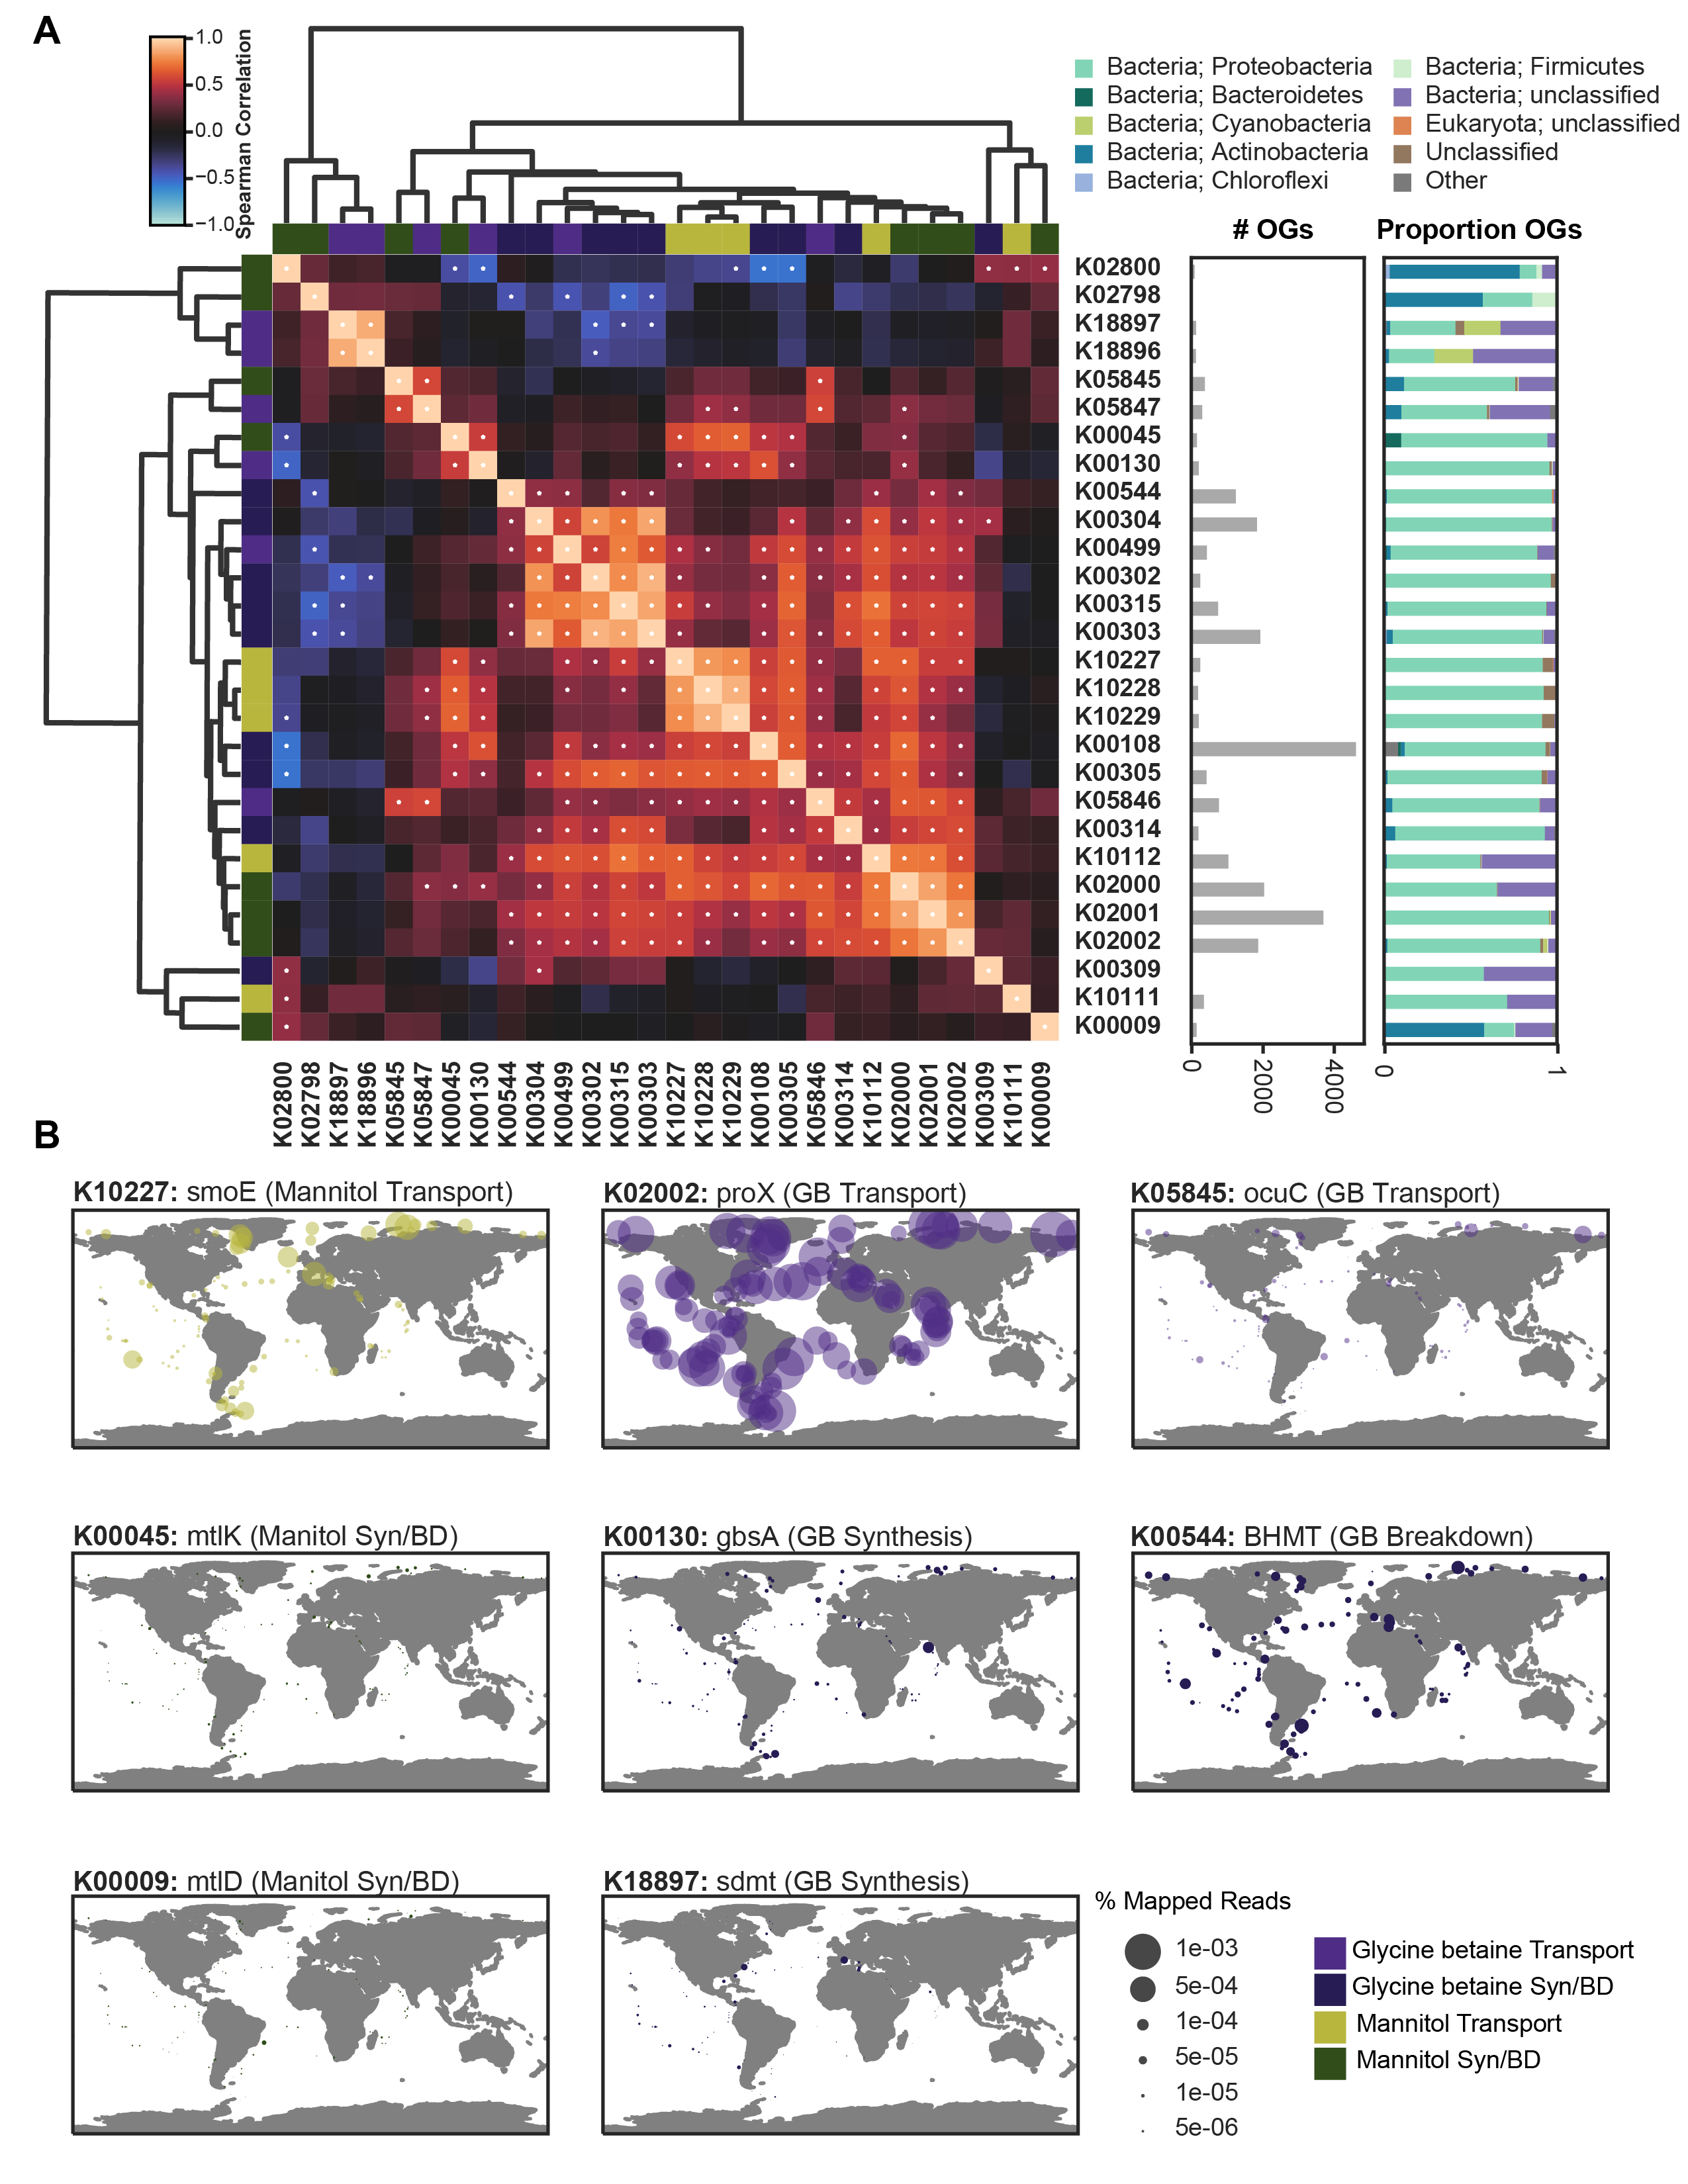
\includegraphics[width=0.75\columnwidth]{Figures/Tara-composite-01.png}
    \caption{The co-occurrence, taxonomic profile, and global abundance of key orthologs involved in the synthesis, breakdown, and transport of mannitol and glycine betaine. The metatranscriptomic abundance of key orthologs involved in the processing of mannitol (green) and glycine betaine (purple) was assessed across the prokaryotic metatranscriptomic data from Tara Oceans using the OM-RGC\_v2 dataset (\Cref{fig:bact-Man}, \ref{fig:bact-GB}). (A) The relative correlation of metatranscriptomic profiles for each of the orthologs considered was assessed by taking the Spearman's correlation of the sum of all orthologs at a given site. The Spearman's $\rho$ is depicted with a heatmap that is clustered based on Bray-Curtis similarity. Significant correlations were determined with a Bonferroni multi-testing p-value correction, and significant correlations (defined as $p<0.001$) are depicted as a white dot. The total number of orthologs (OGs) is depicted as a bar graph and the taxonomic breakdown of the OGs is given as a proportion. (B) The relative abundance of key orthologs of interest is plotted as percent mapped reads across all surface samples from the Tara Oceans sampling efforts. Genes involved in mannitol metabolism include: K10111: malK, K10112: msmK, K10227: smoE, K10228: smoF, K10229: smoG, K00009: mtlD, K00045: mtlK, K02800, mtlA, K02798: cmtB. Genes involved in glycine betaine metabolism include: K02000: proV, K02001: proW,   K02002: proX,  K05845: opuC, K05846: opuBD, K05847: opuA, K00130: gbsA, K00499: CMO, K18896: gsmt, K18897: sdmt, K00108: betA, K00315: DMGDH, K00302: soxA, K00303: soxB, K00304: soxD, K00305: soxG, K00309: dmg, K00544: BHMT, K00314: SARDH.   }
    \label{fig:tarabact}
\end{figure}


\subsection{Metatranscriptomic evidence of osmolyte cycling across the surface ocean}

In addition to assessing the genetic potential for osmolyte metabolism in marine microbe monocultures, the metabolism of two key osmolytes, glycine betaine, an amino acid derivative representative, and mannitol, a sugar representative, across the global ocean was assessed using the Tara prokaryotic and eukaryotic metatranscriptomic data \citep{Salazar_2019, Carradec2018}. We decided to assess the metatranscriptomic signatures of genes associated with targeted osmolytes, as metatranscriptomics provides the ability to assess the transcription and potential activity of these genes across populations  \citep{Alexander2015a, Alexander2020, hu2018, Salazar_2019}. The Ocean Gene Atlas \citep{Villar_2018} was used to assess 1) the diversity of \emph{in situ} communities capable of transport, synthesis, and breakdown of each osmolyte, and 2) the geographical patterns of osmolyte cycling across the surface ocean. Representative KOs were chosen for different subpathways of glycine betaine and mannitol transport, breakdown, and synthesis, and correlations were calculated for the total abundance of orthologs across samples (Supplemental Data Sheet 4). Broadly, we found an alignment in the taxonomic distribution of transcripts recovered with our survey of cultivated genomes and transcriptomes (\Cref{fig:bact} \& \ref{fig:tarabact}A). Additionally, we show that transporters were much more highly abundant in the metatranscriptomic datasets compared to either synthesis or breakdown pathways (\Cref{fig:tarabact}). We also highlight the importance of metazoans in the cycling of glycine betaine (\Cref{fig:tara-meta}). 

Subunits for the different transport systems significantly correlated ($p<0.001$) with each other across samples (\Cref{fig:tarabact} A). Proteobacteria dominated both the total expression and the recovered orthologs of both osmolyte transport systems. For mannitol, the substrate-binding subunit (K10227) and permease subunits (K10228, K10229) of the mannitol transport system cluster together and are significantly correlated ($\rho > 0.79$)  (\Cref{fig:tarabact} A), suggesting that they are co-expressed across the ocean. By contrast, the ATP-binding subunit (K10111, K10112) of the mannitol transport system did not cluster with the other subunits, though one (K10112) was significantly correlated with the associated subunits ($\rho >0.57$) (\Cref{fig:tarabact} A). Two different ABC transporter systems in KEGG are associated with glycine betaine. The glycine betaine/proline transporter is more common than the osmoprotectant transporter (\Cref{fig:tarabact} A). All subunits (K02000, K02001, K02002) for the glycine betaine/proline transport system cluster together and are significantly correlated ($\rho >0.72$). The ATP-binding subunit (K05847) and the substrate-binding subunit (K05845) of the osmoprotectant transporter were significantly correlated ($\rho=0.59$). The permease subunit (K05846) for the osmoprotectant transporter did not cluster with the other subunits, but was significantly correlated with the ATP-binding and substrate-binding subunits ($\rho>0.56$) (\Cref{fig:tarabact} A). 

Mannitol is often recycled internally, and therefore two mannitol-associated KOs (K00045, K00009) were annotated as being capable of both mannitol breakdown and synthesis (recycling). The recycling of mannitol and fructose (K00045) was highly correlated with three subunits of the mannitol transport system ($\rho > 0.60$). Both the expression and recovered orthologs for K00045 were dominated by Proteobacteria, but also included the greatest representation of Bacteroidetes relative to all other KOs (\Cref{fig:tarabact} A). The recycling of mannitol and fructose-6-phosphate (K00009) was not significantly correlated with any other orthologs, except for K02800 ($\rho = 0.41$) (\Cref{fig:tarabact} A). Both the recovered transcripts and expression of mannitol and beta-d-fructose-6-phosphate recycling, as well as the breakdown of mannitol via a phosphotransferase (K02798,K02800), were uniquely dominated by Actinobacteria.
The orthologs for synthesis and breakdown of glycine betaine were overall more abundant than those for mannitol (\Cref{fig:tarabact} B). The methyltransferases involved in glycine betaine synthesis from glycine (K18896) and sarcosine (K18897) were significantly correlated ($\rho=0.88$), and the expression of these orthologs uniquely included a significant portion of Cyanobacteria. Glycine betaine has been previously detected in Cyanobacteria \citep{Fiore2015,Heal2020.12.22.424086}. Specifically, glycine betaine was characterized in \emph{Synechococcus sp.} WH8102 with the two methyltransferases required for synthesis \citep{Lu2006}. The KO for glycine betaine synthesis from choline (K00108) was the most highly expressed (\Cref{fig:bact-GB}). The expression of orthologs associated with this synthesis pathway (K00499, K00108, K00130) were dominated by Proteobacteria, but were not all significantly correlated with each other. The breakdown of glycine betaine to glycine is a three-step pathway and the associated orthologs were all significantly correlated (K00315, K00302, K00303, K00304) ($\rho > 0.73$). This glycine betaine breakdown cluster was almost exclusively expressed by Proteobacteria and was significantly anti-correlated with the orthologs for glycine betaine transport ($\rho > 0.40$) (\Cref{fig:tarabact} A). Interestingly, glycine betaine breakdown was negatively correlated with richness across all samples, suggesting that this pathway is limited to a niche-group, as was observed in the the prokaryotic genomes (\Cref{fig:bact-spearman}, \Cref{fig:bact}).

Globally, the mannitol/sorbitol transporter (K10227) was detected in most samples, but expression levels were particularly high towards the poles (\Cref{fig:tarabact} B). The latitudinal trend was supported by a significant negative correlation between temperature and mannitol/sorbitol transporter expression ($\rho=-0.66$) (\Cref{fig:bact-spearman}). Salinity conditions at the poles are significantly different, and therefore may represent sites of osmolyte recycling that are unique from the majority of the open ocean \citep{Bano2004}. Both mannitol recycling genes (K00045, K00009) were expressed at comparatively low levels (\Cref{fig:tarabact} B, \Cref{fig:bact-Man}). Mannitol is generally not considered to be commonly used by prokaryotes \citep{Empadinhas2008}, but it has been experimentally identified as an osmolyte in several bacteria \citep{Kets1996,Zahid2015}, though not in any marine bacteria. However, marine bacteria clearly transport mannitol (and/or sorbitol) actively, while expression of the associated cellular recycling genes are orders of magnitude lower (\Cref{fig:tarabact} B). While the potential role of mannitol in marine bacteria is not entirely clear, mannitol, like other sugars and polyols, is used as a cryoprotectant in industrial applications where bacterial cells must be preserved through freezing \citep{Savini2010}. We hypothesize that the increased expression of the mannitol/sorbitol transporter in the bacterial size fraction at the poles may be linked to the availability of mannitol through production by eukaryotic phytoplankton, and its cryoprotectant properties for the bacteria. 

Both glycine betaine transporters (the glycine betaine/proline transporter, K02002, and the osmoprotectant transporter, K05845) were present in bacterial transcripts. However, the glycine betaine/proline transporter was much more highly expressed throughout the surface ocean and did not show any clear differentiation between high and low latitudes or temperature (\Cref{fig:tarabact} B, \Cref{fig:bact-spearman}). This expression was predominantly derived from unknown or unclassified bacteria and Proteobacteria. Previous work has shown that the Proteobacteria SAR11 have a high-affinity glycine betaine transporter \citep{Noell2019}. \emph{Vibrio parahaemolyticus} species contains two proU ABC transporters, but have also been found to transport glycine betaine, along with dimethylglycine, choline, ectoine, and proline with a BCCT transporter which was not linked to glycine betaine in KEGG \citep{Gregory2020}. Unlike mannitol, a glycine betaine breakdown gene (K00544) was expressed at an order of magnitude higher than the synthesis gene (K18897), and was, again, predominantly expressed by Proteobacteria (\Cref{fig:tarabact} B, \Cref{fig:bact-GB}). The glycine betaine transport and breakdown expressions suggests that after transport into the cell, glycine betaine may be more commonly recycled through anabolic pathways or catabolized, rather than used as an osmolyte, at least compared to mannitol. Proteobacteria appear to be the most significant prokaryotic group metabolizing glycine betaine in Tara. Nanomolar concentrations of glycine betaine are rapidly scavenged from seawater, and most of this activity is assumed to be driven by bacteria (in the $<1\mu m$ fraction) \citep{Kiene1998}. Radiolabeled glycine betaine was rapidly incorporated in its existing molecular structure, but after 46 hours of incubation, 46\% of the radioactivity was transformed into carbon dioxide \citep{Kiene1998}, indicating substantial remineralization of glycine betaine as a carbon (and possibly a nitrogen) substrate.
\begin{figure}[t!]
    \centering
    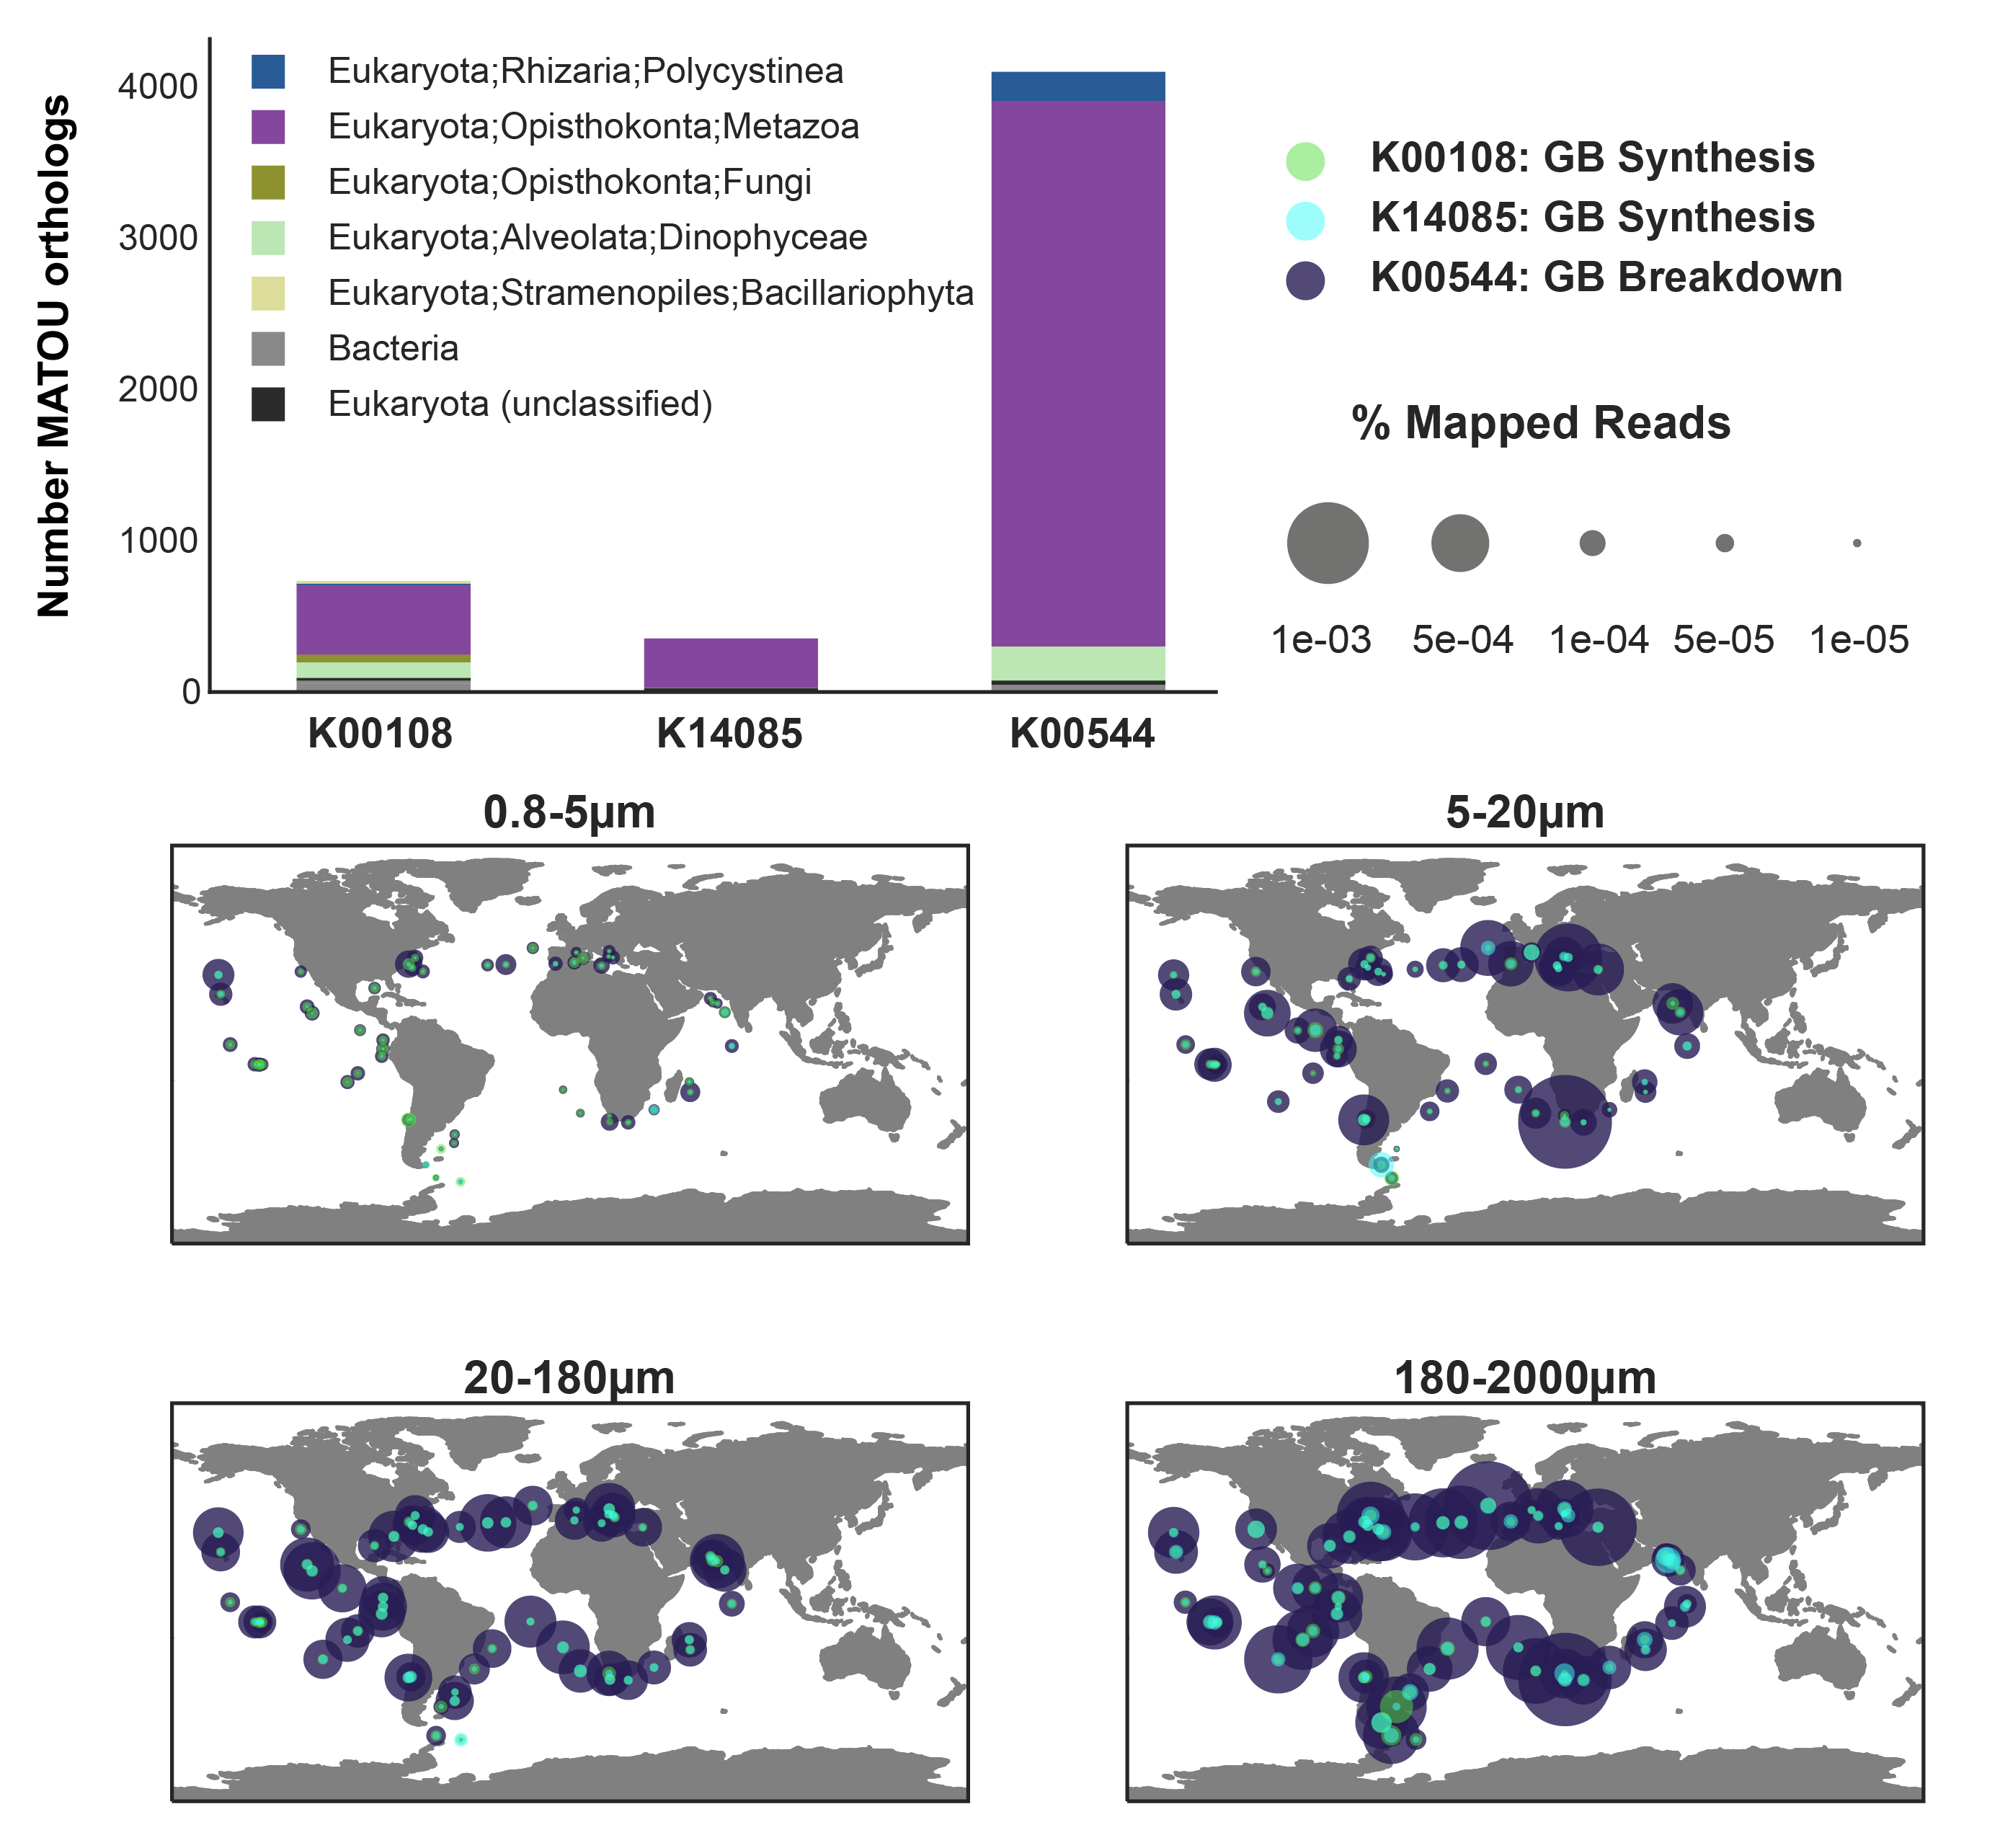
\includegraphics[width=0.85\columnwidth]{Figures/Euk_K00544_GBbreakdown-01.png}
    \caption{The abundance and diversity of KOs associated with the synthesis and breakdown of glycine betaine across eukaryotic metatranscriptomic data from Tara Oceans. Genes included in the analysis include: Betaine-homocysteine S-methyltransferase (K00544), a central enzyme for the breakdown of glycine betaine, 4267 orthologs of K00544 were identified in the MATOU-v1 dataset; choline dehydrogenase (K00108), 826 orthologs recovered; aldehyde dehydrogenase A1 (K14085), 384 orthologs recovered. (A) The taxonomic breakdown of the orthologs as published in MATOU-v1 is depicted as stacked bar plot (top). (B) The relative abundance of the three KOs (\Cref{fig:euk-GB}, \ref{fig:euk-Man}) in the eukaryotic metatranscriptome dataset from the surface ocean in Tara is shown by size fraction ($0.8-5 \mu m, 5-20 \mu m, 20-180 \mu m$, and $180-2000\mu m$).}
    \label{fig:tara-meta}
\end{figure}

\subsection{Zooplankton and the cycling of glycine betaine}


Glycine betaine synthesis and breakdown was also present in eukaryotic unigenes \citep{Carradec2018}. The taxonomy of glycine betaine synthesis (K00108, K14085) and breakdown was dominated by Arthropoda (specifically, copepods), but was also found in Vertebrata (fish) and protists (Dinophyceae and Rhizaria) (\Cref{fig:tara-meta}). A similar protistan signature was observed in MMETSP transcriptomes, where glycine betaine breakdown was exclusively observed in Dinophyceae (Alveolata) (\Cref{fig:euk}). The observation of Rhizaria capable of glycine betaine breakdown (\Cref{fig:tara-meta}) likely results from Rhizaria (Polycystinea) transcriptomes that were used to supplement the MMETSP transcriptomes as references for taxonomy assignment in the MATOU \citep{Carradec2018}. Additionally, genes for glycine betaine synthesis from glycine (K18896, K24071) in Tara were positively correlated with the Dinophyceae pigment marker ($\rho > 0.22$), peridinin, across all samples (\Cref{fig:euk-spearman}). As was observed in prokaryotes (\Cref{fig:tarabact}), glycine betaine synthesis from choline was also most abundant across eukaryotes (\Cref{fig:euk-GB}). However, across all size fractions, total expression by eukaryotes was dominated by glycine betaine breakdown to glycine (\Cref{fig:tara-meta}). The protist contribution to glycine betaine breakdown expression is most likely represented in the $5-20\mu m$, whereas the highest expression was contributed by the Arthropoda and Vertebrata in the $180-2000\mu m$ fraction.

Copepod excretion is a potentially important source of labile substrates \citep{Maas2020}. Previous studies have described taurine as an important osmolyte in marine copepods \citep{Clifford2020}. Although glycine betaine has been described across all three domains of life \citep{Yancey2005}, to our knowledge, the potential for glycine betaine synthesis and breakdown has not been described previously for marine planktonic Arthropoda. The expression patterns described here for eukaryotic unigenes hint at an important role for not only protists, but also higher-order marine eukaryotes in the recycling of this osmolyte. The disconnect between breakdown and synthesis across all eukaryotic size fractions suggests that eukaryotes are capable of obtaining glycine betaine from the environment. In the case of multicellular organisms, glycine betaine could be obtained through grazing or the microbiome \citep{Shoemaker2017}. The dominance of breakdown could in part be due to the conservative threshold used here to filter ortholog hits causing a higher recovery of breakdown KOs and/or removal of synthesis genes. The expression of both synthesis and breakdown of glycine betaine in the $180-2000 \mu m$ fraction suggests that multicellular organisms, particularly copepods, could be an important source or sink of this osmolyte that is not currently considered.

\section{Conclusions}

Osmolytes are core cellular metabolites that are required for all marine microbes living in the high salinity environment of the ocean. Across the three domains of life, we found that osmolyte metabolic capabilities could be broken down into two main categories: 1) globally ubiquitous, and 2) mosaically present across groups. The synthesis and breakdown of three amino acid osmolytes surveyed (glutamate, glutamine, and proline) were common across all prokaryotes and eukaryotes. The ubiquity of synthesis and breakdown of these core metabolites likely indicates an important role for internal recycling. Although it is difficult to directly attribute osmotic function without experimental evidence, we hypothesized that osmolytes in genomes with synthesis only, or genomes with transport only were more likely used for osmotic functions. The genomic evidence for a potential osmotic function (synthesis or transport in the absence of breakdown) was most apparent for the classically known osmolyte, glycine betaine, which appeared to be a unique instance of osmolyte specificity in the absence of central metabolic importance. The dominance of synthesis or breakdown of the other osmolytes surveyed differed significantly across prokaryotes and eukaryotes, suggesting that osmolyte sources and sinks are taxa dependent. Critically, the ability to breakdown was most common relative to synthesis or transport for the majority of the osmolytes surveyed, suggesting that these small molecules serve a central metabolic function and are likely important substrates in the microbial loop.

We took a two pronged approach in our survey of osmolyte metabolism within marine taxa: 1) examining metabolic potential within reference genomes and transcriptomes and 2) assessing transcriptional activity from mixed communities across the global ocean. When we compared the potential of taxonomic groups to synthesize, breakdown, and transport osmolytes to the expression of the genes associated with these pathways in the environmental metatranscriptomic data, we found good agreement between the species with the potential to perform these metabolic functions, and those that were observed to transcribe the relevant genes in the environment. In the environment, bacterial transcription of transporter genes for both mannitol and glycine betaine were an order of magnitude higher than their respective genes for synthesis and breakdown. Although only four Alphaproteobacteria genomes were found to have the potential for glycine betaine breakdown, the relative abundance of transcription of the breakdown pathway was significantly higher than the breakdown pathway for mannitol. One of the strains capable of breakdown of glycine betaine, Candidatus \emph{Pelagibacter ubique}, is a highly abundant taxa found broadly throughout the oligotrophic ocean \citep{Morris2002}, which perhaps explains the high level of transcription. This suggests that a niche based on glycine betaine as a carbon source may be occupied by these species without competition from other bacterial species. Interestingly, although synthesis of glycine betaine by eukaryotic size fractions was widespread, breakdown was most highly expressed in the larger size fractions, particularly by metazoa. Thus, not only are protists likely important sinks of the osmolyte glycine betaine, but also higher-order, multicellular eukaryotes should also be considered as potential sinks. This finding  would not have been possible without probing the Tara metatranscriptomes. Our initial investigation of two key osmolytes within the Tara metatranscriptomes highlights the fact that both eukaryotes and prokaryotes are actively using and recycling osmolytes \emph{in situ}, and that osmolytes are potentially being exchanged between pelagic bacteria, phytoplankton, and also zooplankton. Marine protists, particularly phytoplankton, are most often emphasized as potential sources of marine osmolytes, but clearly connections with higher order trophic levels are also important in the global cycling of carbon and should be examined more in depth \citep{Durham2019,Clifford2020}.

The ocean is a dynamic and variable environment, and the organisms that inhabit it must be prepared to survive sudden environmental fluctuations. Here we surveyed and reviewed the osmoadaptive capabilities in the form of the synthesis, breakdown, and transport of various osmolytes across cultured organisms with sequenced genomes or transcriptomes as well as within a global metatranscriptomic dataset. We believe that the work here serves as a first step in the targeted and informed examination of osmoregulation by ecologically-relevant groups in the microbial loop. In particular, further work examining the presence and absence of these genes across metagenome assembled genomes (MAGs) or single celled amplified genomes (SAGs) may provide greater insights into the osmoadaptive capabilities of uncultivated lineages. Additionally, examining rates of uptake and loss of osmolytes from cells, coupled with more comprehensive characterization of their dissolved concentrations in the ocean, would support our understanding of their potentially significant influence on labile carbon cycling in the ocean. Broadly, we show that while some osmolytes (e.g. the amino acids glutamate and glutamine) are ubiquitously synthesized and broken down across the tree of life, the ability to synthesize, breakdown, and transport most osmolytes is present mosaically across organisms. The mosaicism of the genomic traits of osmolyte metabolism may suggest that many of the osmolytes surveyed here are central currencies of exchange between organisms \citep{Moran2016}, between domains or within domains. 

\bgroup
\def\arraystretch{1.5}%
\begin{landscape}
\begin{table}[]
\begin{tabular}{llllllll}
\textbf{Common name} & \textbf{g/mol} & \textbf{Category} & \textbf{N atoms} & \textbf{S atoms} & \textbf{Cellular} & \textbf{Dissolved (nM)} & \\ \hline
trigonelline         & 137            & alkaloid          & 0                & 1                & +                 & -                                   \\
\textbf{TMAO}                 & 75             & amine oxide       & 1                & 0                & +                 & 2-77 \citep{Hatton1999,Gibb2004}     \\
\textbf{ectoine}              & 142            & amino acid        & 2                & 0                & +                 & 0.1-0.3 \citep{Widner2021}              \\
\textbf{GABA}                 & 103            & amino acid        & 1                & 0                & +                 & 0.1 \citep{Widner2021}              \\
\textbf{glutamate}            & 147            & amino acid        & 1                & 0                & +                 & 0.7-5 \citep{Widner2021,Mopper1982}   \\
\textbf{glutamine}            & 146            & amino acid        & 2                & 0                & +                 & 0.2-3 \citep{Widner2021,Mopper1982}   \\
\textbf{glycine betaine}      & 117            & amino acid        & 1                & 0                & +                 & -                                       \\
homarine             & 137            & amino acid        & 1                & 0                & +                 & -                                      \\
homoserine betaine   & 161            & amino acid        & 1                & 0                & +                 & -                                       \\
hydroxyectoine       & 158            & amino acid        & 2                & 0                & +                 & -                                        \\
\textbf{proline}              & 115            & amino acid        & 1                & 0                & +                 & 0.4 \citep{Widner2021}              \\
\textbf{sarcosine}            & 89             & amino acid        & 1                & 0                & +                 & 0.1-0.2 \citep{Widner2021}              \\
\textbf{taurine}              & 125            & amino acid        & 1                & 1                & +                 & 0.1-320 \citep{Widner2021,Clifford2017} \\
glucosylglycerol     & 254            & sugar             & 0                & 0                & +                 & -                                        \\
isofloridoside       & 254            & sugar             & 0                & 0                & +                 & -                                         \\
\textbf{sucrose}              & 342            & sugar             & 0                & 0                & +                 & BD \citep{Sakugawa1985}                                         \\
\textbf{trehalose}            & 342            & sugar             & 0                & 0                & +                 & BD \citep{Sakugawa1985}                                         \\
\textbf{glycerol}             & 92             & sugar alcohol     & 0                & 0                & +                 & -                                          \\
\textbf{mannitol}             & 182            & sugar alcohol     & 0                & 0                & +                 & -                                          \\
\textbf{sorbitol}             & 182            & sugar alcohol     & 0                & 0                & +                 & -                                          \\
DHPS                 & 155            & sulfonate         & 0                & 1                & +                 & 0.26-0.44 \citep{Widner2021}              \\
DMSP                 & 134            & sulfonium         & 0                & 1                & +                 & 1-2 \citep{Kiene2006}               \\
gonyol               & 178            & sulfonium         & 0                & 1                & +                 & -                                                                         
\end{tabular}
\caption{Osmolytes previously described in marine microbes. The table includes: Common name of osmolyte, molecular weight (g/mol), nominal category, number of nitrogen (N) atoms, number of sulfur (S) atoms, cellular concentrations reported (+) in monocultures, and previously measured dissolved concentrations (nM) from coastal or open ocean environments. Names in bold were used in the analyses presented here. As osmolyte cellular concentrations are extremely variable, we only report if an osmolyte has been previously reported in monocultures \citep{Dickson1987,Dickson1987.2,Brown1978,Keller1989,Pade2012,Pade2016,Gebser2013,Durham2019,Fenizia2020,Yancey2005,Mountfort1992,Reed1986,Lin2020}. To our knowledge, dissolved measurements of most osmolytes do not exist. Abbreviations: GABA = 4-aminobutanoate, TMAO = trimethylamine n-oxide, DMSP = dimethylsulfoniopropionate, DHPS = dihydroxypropane-sulfonate, BD = below detection}
\label{tabl:osmodiss}
\end{table}
\end{landscape}
\egroup

\bgroup
\def\arraystretch{1.5}%

\begin{table}
\begin{tabular}{lllll}
\noalign{\global\arrayrulewidth=2pt}
\textbf{Common name} & \textbf{KEGG id} & \multicolumn{1}{l}{\textbf{Breakdown}} & \multicolumn{1}{l}{\textbf{Synthesis}} & \multicolumn{1}{l}{\textbf{Transport}} \\ \hline
ectoine              & C06231           & 2 \emph{(1-3)}                                & 2 \emph{(4-5)}                                & 0                                      \\
GABA                 & C00334           & 4 \emph{(1-2)}                                & 11 \emph{(1-4)}                               & 0                                      \\
glutamate            & C00025           & 61 \emph{(1-5)}                               & 78 \emph{(1-3)}                               & 0                                      \\
glutamine            & C00064           & 30 \emph{(1)}                                 & 2 \emph{(1)}                                  & 0                                      \\
glycine betaine      & C00719           & 1 \emph{(3)}                                  & 4 \emph{(1-2)}                                & 2 \emph{(3)}                                  \\
proline              & C00148           & 12 \emph{(1)}                                 & 6 \emph{(1-2)}                                & 0                                      \\
sarcosine            & C00213           & 2 \emph{(1)}                                  & 7 \emph{(1-4)}                                & 0                                      \\
taurine              & C00245           & 6 \emph{(1)}                                  & 5 \emph{(1)}                                  & 1 \emph{(3)}                                  \\
glycerol             & C00116           & 7 \emph{(1-3)}                                & 9 \emph{(1-4)}                                & 1 \emph{(3)}                                  \\
mannitol             & C00392           & 2 \emph{(1-2)}                                & 1 \emph{(2)}                                  & 1 \emph{(3)}                                  \\
sorbitol             & C00794           & 4 \emph{(1)}                                  & 4 \emph{(1)}                                  & 1 \emph{(3)}                                   \\
sucrose              & C00089           & 12 \emph{(1)}                                 & 3 \emph{(1-3)}                                & 0                                      \\
trehalose            & C01083           & 6 \emph{(1)}                                  & 5 \emph{(1-3)}                                & 0                                      \\
TMAO                 & C01104           & 1 \emph{(1)}                                  & 1 \emph{(1)}                                  & 0                                     
\end{tabular}
\caption{Osmolytes included in prokaryote and eukaryote surveys. The table includes: Common name of osmolyte, the KEGG ID, the total number of curated pathways with associated KOs used in the searches for breakdown, synthesis, and transport, and the range of steps in each pathway in parentheses. Some pathways required the presence of multiple steps (i.e. KOs) to be considered complete (Supplemental Data Sheet 1). A single step value indicates all pathways had the same number of steps. For osmolyte pathways with differing number of steps, a range is reported which reflects the minimum and maximum number of steps for all pathways. Abbreviations: GABA = 4-aminobutanoate, TMAO =  trimethylamine n-oxide}
\label{tabl:pathnum}
\end{table}
\egroup


\section*{Conflict of Interest Statement}
%All financial, commercial or other relationships that might be perceived by the academic community as representing a potential conflict of interest must be disclosed. If no such relationship exists, authors will be asked to confirm the following statement: 

The authors declare that the research was conducted in the absence of any commercial or financial relationships that could be construed as a potential conflict of interest.

\section*{Author Contributions}
All three authors contributed equally to the development of this project, analysis of the data, and writing of the manuscript.

\section*{Funding}
ELM was supported by the Postdoctoral Scholar Program at Woods Hole Oceanographic Institution. WMJ was supported by a Research Initiative Award from the College of Arts and Sciences at the University of North Carolina Wilmington. HA was supported by a Independent Research and Development Award from the Woods Hole Oceanographic Institution. 

\section*{Acknowledgments}
This research would not have been possible without the community driven efforts to provide open and freely available data by the Tara Oceans Consortium, the Marine Microbial Transcriptome Sequencing Project (MMETSP), the Marine Metagenomics Portal, and the Kyoto Encyclopedia of Genes and Genomes (KEGG).  
\section*{Data Availability Statement}
These analyses were based on previously existing datasets including the MMETSP (\url{https://zenodo.org/record/1212585}), Tara Oceans Gene Atlas (\url{https://tara-oceans.mio.osupytheas.fr/ocean-gene-atlas/}), KEGG homologs (\url{https://www.genome.jp/tools/kofamkoala/}), and MarRef v5 (\url{https://mmp.sfb.uit.no/downloads/}). 


\bibliographystyle{frontiersinSCNS_ENG_HUMS} % for Science, Engineering and Humanities and Social Sciences articles, for Humanities and Social Sciences articles please include page numbers in the in-text citations
%\bibliographystyle{frontiersinHLTH&FPHY} % for Health, Physics and Mathematics articles
\bibliography{main}

%%% Make sure to upload the bib file along with the tex file and PDF
%%% Please see the test.bib file for some examples of references


\end{document}
